
% Default to the notebook output style

    


% Inherit from the specified cell style.




    
\documentclass[11pt]{article}

    
    
    \usepackage[T1]{fontenc}
    % Nicer default font (+ math font) than Computer Modern for most use cases
    \usepackage{mathpazo}

    % Basic figure setup, for now with no caption control since it's done
    % automatically by Pandoc (which extracts ![](path) syntax from Markdown).
    \usepackage{graphicx}
    % We will generate all images so they have a width \maxwidth. This means
    % that they will get their normal width if they fit onto the page, but
    % are scaled down if they would overflow the margins.
    \makeatletter
    \def\maxwidth{\ifdim\Gin@nat@width>\linewidth\linewidth
    \else\Gin@nat@width\fi}
    \makeatother
    \let\Oldincludegraphics\includegraphics
    % Set max figure width to be 80% of text width, for now hardcoded.
    \renewcommand{\includegraphics}[1]{\Oldincludegraphics[width=.8\maxwidth]{#1}}
    % Ensure that by default, figures have no caption (until we provide a
    % proper Figure object with a Caption API and a way to capture that
    % in the conversion process - todo).
    \usepackage{caption}
    \DeclareCaptionLabelFormat{nolabel}{}
    \captionsetup{labelformat=nolabel}

    \usepackage{adjustbox} % Used to constrain images to a maximum size 
    \usepackage{xcolor} % Allow colors to be defined
    \usepackage{enumerate} % Needed for markdown enumerations to work
    \usepackage{geometry} % Used to adjust the document margins
    \usepackage{amsmath} % Equations
    \usepackage{amssymb} % Equations
    \usepackage{textcomp} % defines textquotesingle
    % Hack from http://tex.stackexchange.com/a/47451/13684:
    \AtBeginDocument{%
        \def\PYZsq{\textquotesingle}% Upright quotes in Pygmentized code
    }
    \usepackage{upquote} % Upright quotes for verbatim code
    \usepackage{eurosym} % defines \euro
    \usepackage[mathletters]{ucs} % Extended unicode (utf-8) support
    \usepackage[utf8x]{inputenc} % Allow utf-8 characters in the tex document
    \usepackage{fancyvrb} % verbatim replacement that allows latex
    \usepackage{grffile} % extends the file name processing of package graphics 
                         % to support a larger range 
    % The hyperref package gives us a pdf with properly built
    % internal navigation ('pdf bookmarks' for the table of contents,
    % internal cross-reference links, web links for URLs, etc.)
    \usepackage{hyperref}
    \usepackage{longtable} % longtable support required by pandoc >1.10
    \usepackage{booktabs}  % table support for pandoc > 1.12.2
    \usepackage[inline]{enumitem} % IRkernel/repr support (it uses the enumerate* environment)
    \usepackage[normalem]{ulem} % ulem is needed to support strikethroughs (\sout)
                                % normalem makes italics be italics, not underlines
    

    
    
    % Colors for the hyperref package
    \definecolor{urlcolor}{rgb}{0,.145,.698}
    \definecolor{linkcolor}{rgb}{.71,0.21,0.01}
    \definecolor{citecolor}{rgb}{.12,.54,.11}

    % ANSI colors
    \definecolor{ansi-black}{HTML}{3E424D}
    \definecolor{ansi-black-intense}{HTML}{282C36}
    \definecolor{ansi-red}{HTML}{E75C58}
    \definecolor{ansi-red-intense}{HTML}{B22B31}
    \definecolor{ansi-green}{HTML}{00A250}
    \definecolor{ansi-green-intense}{HTML}{007427}
    \definecolor{ansi-yellow}{HTML}{DDB62B}
    \definecolor{ansi-yellow-intense}{HTML}{B27D12}
    \definecolor{ansi-blue}{HTML}{208FFB}
    \definecolor{ansi-blue-intense}{HTML}{0065CA}
    \definecolor{ansi-magenta}{HTML}{D160C4}
    \definecolor{ansi-magenta-intense}{HTML}{A03196}
    \definecolor{ansi-cyan}{HTML}{60C6C8}
    \definecolor{ansi-cyan-intense}{HTML}{258F8F}
    \definecolor{ansi-white}{HTML}{C5C1B4}
    \definecolor{ansi-white-intense}{HTML}{A1A6B2}

    % commands and environments needed by pandoc snippets
    % extracted from the output of `pandoc -s`
    \providecommand{\tightlist}{%
      \setlength{\itemsep}{0pt}\setlength{\parskip}{0pt}}
    \DefineVerbatimEnvironment{Highlighting}{Verbatim}{commandchars=\\\{\}}
    % Add ',fontsize=\small' for more characters per line
    \newenvironment{Shaded}{}{}
    \newcommand{\KeywordTok}[1]{\textcolor[rgb]{0.00,0.44,0.13}{\textbf{{#1}}}}
    \newcommand{\DataTypeTok}[1]{\textcolor[rgb]{0.56,0.13,0.00}{{#1}}}
    \newcommand{\DecValTok}[1]{\textcolor[rgb]{0.25,0.63,0.44}{{#1}}}
    \newcommand{\BaseNTok}[1]{\textcolor[rgb]{0.25,0.63,0.44}{{#1}}}
    \newcommand{\FloatTok}[1]{\textcolor[rgb]{0.25,0.63,0.44}{{#1}}}
    \newcommand{\CharTok}[1]{\textcolor[rgb]{0.25,0.44,0.63}{{#1}}}
    \newcommand{\StringTok}[1]{\textcolor[rgb]{0.25,0.44,0.63}{{#1}}}
    \newcommand{\CommentTok}[1]{\textcolor[rgb]{0.38,0.63,0.69}{\textit{{#1}}}}
    \newcommand{\OtherTok}[1]{\textcolor[rgb]{0.00,0.44,0.13}{{#1}}}
    \newcommand{\AlertTok}[1]{\textcolor[rgb]{1.00,0.00,0.00}{\textbf{{#1}}}}
    \newcommand{\FunctionTok}[1]{\textcolor[rgb]{0.02,0.16,0.49}{{#1}}}
    \newcommand{\RegionMarkerTok}[1]{{#1}}
    \newcommand{\ErrorTok}[1]{\textcolor[rgb]{1.00,0.00,0.00}{\textbf{{#1}}}}
    \newcommand{\NormalTok}[1]{{#1}}
    
    % Additional commands for more recent versions of Pandoc
    \newcommand{\ConstantTok}[1]{\textcolor[rgb]{0.53,0.00,0.00}{{#1}}}
    \newcommand{\SpecialCharTok}[1]{\textcolor[rgb]{0.25,0.44,0.63}{{#1}}}
    \newcommand{\VerbatimStringTok}[1]{\textcolor[rgb]{0.25,0.44,0.63}{{#1}}}
    \newcommand{\SpecialStringTok}[1]{\textcolor[rgb]{0.73,0.40,0.53}{{#1}}}
    \newcommand{\ImportTok}[1]{{#1}}
    \newcommand{\DocumentationTok}[1]{\textcolor[rgb]{0.73,0.13,0.13}{\textit{{#1}}}}
    \newcommand{\AnnotationTok}[1]{\textcolor[rgb]{0.38,0.63,0.69}{\textbf{\textit{{#1}}}}}
    \newcommand{\CommentVarTok}[1]{\textcolor[rgb]{0.38,0.63,0.69}{\textbf{\textit{{#1}}}}}
    \newcommand{\VariableTok}[1]{\textcolor[rgb]{0.10,0.09,0.49}{{#1}}}
    \newcommand{\ControlFlowTok}[1]{\textcolor[rgb]{0.00,0.44,0.13}{\textbf{{#1}}}}
    \newcommand{\OperatorTok}[1]{\textcolor[rgb]{0.40,0.40,0.40}{{#1}}}
    \newcommand{\BuiltInTok}[1]{{#1}}
    \newcommand{\ExtensionTok}[1]{{#1}}
    \newcommand{\PreprocessorTok}[1]{\textcolor[rgb]{0.74,0.48,0.00}{{#1}}}
    \newcommand{\AttributeTok}[1]{\textcolor[rgb]{0.49,0.56,0.16}{{#1}}}
    \newcommand{\InformationTok}[1]{\textcolor[rgb]{0.38,0.63,0.69}{\textbf{\textit{{#1}}}}}
    \newcommand{\WarningTok}[1]{\textcolor[rgb]{0.38,0.63,0.69}{\textbf{\textit{{#1}}}}}
    
    
    % Define a nice break command that doesn't care if a line doesn't already
    % exist.
    \def\br{\hspace*{\fill} \\* }
    % Math Jax compatability definitions
    \def\gt{>}
    \def\lt{<}
    % Document parameters
    \title{e91\_quantum\_key\_distribution\_protocol}
    
    
    

    % Pygments definitions
    
\makeatletter
\def\PY@reset{\let\PY@it=\relax \let\PY@bf=\relax%
    \let\PY@ul=\relax \let\PY@tc=\relax%
    \let\PY@bc=\relax \let\PY@ff=\relax}
\def\PY@tok#1{\csname PY@tok@#1\endcsname}
\def\PY@toks#1+{\ifx\relax#1\empty\else%
    \PY@tok{#1}\expandafter\PY@toks\fi}
\def\PY@do#1{\PY@bc{\PY@tc{\PY@ul{%
    \PY@it{\PY@bf{\PY@ff{#1}}}}}}}
\def\PY#1#2{\PY@reset\PY@toks#1+\relax+\PY@do{#2}}

\expandafter\def\csname PY@tok@w\endcsname{\def\PY@tc##1{\textcolor[rgb]{0.73,0.73,0.73}{##1}}}
\expandafter\def\csname PY@tok@c\endcsname{\let\PY@it=\textit\def\PY@tc##1{\textcolor[rgb]{0.25,0.50,0.50}{##1}}}
\expandafter\def\csname PY@tok@cp\endcsname{\def\PY@tc##1{\textcolor[rgb]{0.74,0.48,0.00}{##1}}}
\expandafter\def\csname PY@tok@k\endcsname{\let\PY@bf=\textbf\def\PY@tc##1{\textcolor[rgb]{0.00,0.50,0.00}{##1}}}
\expandafter\def\csname PY@tok@kp\endcsname{\def\PY@tc##1{\textcolor[rgb]{0.00,0.50,0.00}{##1}}}
\expandafter\def\csname PY@tok@kt\endcsname{\def\PY@tc##1{\textcolor[rgb]{0.69,0.00,0.25}{##1}}}
\expandafter\def\csname PY@tok@o\endcsname{\def\PY@tc##1{\textcolor[rgb]{0.40,0.40,0.40}{##1}}}
\expandafter\def\csname PY@tok@ow\endcsname{\let\PY@bf=\textbf\def\PY@tc##1{\textcolor[rgb]{0.67,0.13,1.00}{##1}}}
\expandafter\def\csname PY@tok@nb\endcsname{\def\PY@tc##1{\textcolor[rgb]{0.00,0.50,0.00}{##1}}}
\expandafter\def\csname PY@tok@nf\endcsname{\def\PY@tc##1{\textcolor[rgb]{0.00,0.00,1.00}{##1}}}
\expandafter\def\csname PY@tok@nc\endcsname{\let\PY@bf=\textbf\def\PY@tc##1{\textcolor[rgb]{0.00,0.00,1.00}{##1}}}
\expandafter\def\csname PY@tok@nn\endcsname{\let\PY@bf=\textbf\def\PY@tc##1{\textcolor[rgb]{0.00,0.00,1.00}{##1}}}
\expandafter\def\csname PY@tok@ne\endcsname{\let\PY@bf=\textbf\def\PY@tc##1{\textcolor[rgb]{0.82,0.25,0.23}{##1}}}
\expandafter\def\csname PY@tok@nv\endcsname{\def\PY@tc##1{\textcolor[rgb]{0.10,0.09,0.49}{##1}}}
\expandafter\def\csname PY@tok@no\endcsname{\def\PY@tc##1{\textcolor[rgb]{0.53,0.00,0.00}{##1}}}
\expandafter\def\csname PY@tok@nl\endcsname{\def\PY@tc##1{\textcolor[rgb]{0.63,0.63,0.00}{##1}}}
\expandafter\def\csname PY@tok@ni\endcsname{\let\PY@bf=\textbf\def\PY@tc##1{\textcolor[rgb]{0.60,0.60,0.60}{##1}}}
\expandafter\def\csname PY@tok@na\endcsname{\def\PY@tc##1{\textcolor[rgb]{0.49,0.56,0.16}{##1}}}
\expandafter\def\csname PY@tok@nt\endcsname{\let\PY@bf=\textbf\def\PY@tc##1{\textcolor[rgb]{0.00,0.50,0.00}{##1}}}
\expandafter\def\csname PY@tok@nd\endcsname{\def\PY@tc##1{\textcolor[rgb]{0.67,0.13,1.00}{##1}}}
\expandafter\def\csname PY@tok@s\endcsname{\def\PY@tc##1{\textcolor[rgb]{0.73,0.13,0.13}{##1}}}
\expandafter\def\csname PY@tok@sd\endcsname{\let\PY@it=\textit\def\PY@tc##1{\textcolor[rgb]{0.73,0.13,0.13}{##1}}}
\expandafter\def\csname PY@tok@si\endcsname{\let\PY@bf=\textbf\def\PY@tc##1{\textcolor[rgb]{0.73,0.40,0.53}{##1}}}
\expandafter\def\csname PY@tok@se\endcsname{\let\PY@bf=\textbf\def\PY@tc##1{\textcolor[rgb]{0.73,0.40,0.13}{##1}}}
\expandafter\def\csname PY@tok@sr\endcsname{\def\PY@tc##1{\textcolor[rgb]{0.73,0.40,0.53}{##1}}}
\expandafter\def\csname PY@tok@ss\endcsname{\def\PY@tc##1{\textcolor[rgb]{0.10,0.09,0.49}{##1}}}
\expandafter\def\csname PY@tok@sx\endcsname{\def\PY@tc##1{\textcolor[rgb]{0.00,0.50,0.00}{##1}}}
\expandafter\def\csname PY@tok@m\endcsname{\def\PY@tc##1{\textcolor[rgb]{0.40,0.40,0.40}{##1}}}
\expandafter\def\csname PY@tok@gh\endcsname{\let\PY@bf=\textbf\def\PY@tc##1{\textcolor[rgb]{0.00,0.00,0.50}{##1}}}
\expandafter\def\csname PY@tok@gu\endcsname{\let\PY@bf=\textbf\def\PY@tc##1{\textcolor[rgb]{0.50,0.00,0.50}{##1}}}
\expandafter\def\csname PY@tok@gd\endcsname{\def\PY@tc##1{\textcolor[rgb]{0.63,0.00,0.00}{##1}}}
\expandafter\def\csname PY@tok@gi\endcsname{\def\PY@tc##1{\textcolor[rgb]{0.00,0.63,0.00}{##1}}}
\expandafter\def\csname PY@tok@gr\endcsname{\def\PY@tc##1{\textcolor[rgb]{1.00,0.00,0.00}{##1}}}
\expandafter\def\csname PY@tok@ge\endcsname{\let\PY@it=\textit}
\expandafter\def\csname PY@tok@gs\endcsname{\let\PY@bf=\textbf}
\expandafter\def\csname PY@tok@gp\endcsname{\let\PY@bf=\textbf\def\PY@tc##1{\textcolor[rgb]{0.00,0.00,0.50}{##1}}}
\expandafter\def\csname PY@tok@go\endcsname{\def\PY@tc##1{\textcolor[rgb]{0.53,0.53,0.53}{##1}}}
\expandafter\def\csname PY@tok@gt\endcsname{\def\PY@tc##1{\textcolor[rgb]{0.00,0.27,0.87}{##1}}}
\expandafter\def\csname PY@tok@err\endcsname{\def\PY@bc##1{\setlength{\fboxsep}{0pt}\fcolorbox[rgb]{1.00,0.00,0.00}{1,1,1}{\strut ##1}}}
\expandafter\def\csname PY@tok@kc\endcsname{\let\PY@bf=\textbf\def\PY@tc##1{\textcolor[rgb]{0.00,0.50,0.00}{##1}}}
\expandafter\def\csname PY@tok@kd\endcsname{\let\PY@bf=\textbf\def\PY@tc##1{\textcolor[rgb]{0.00,0.50,0.00}{##1}}}
\expandafter\def\csname PY@tok@kn\endcsname{\let\PY@bf=\textbf\def\PY@tc##1{\textcolor[rgb]{0.00,0.50,0.00}{##1}}}
\expandafter\def\csname PY@tok@kr\endcsname{\let\PY@bf=\textbf\def\PY@tc##1{\textcolor[rgb]{0.00,0.50,0.00}{##1}}}
\expandafter\def\csname PY@tok@bp\endcsname{\def\PY@tc##1{\textcolor[rgb]{0.00,0.50,0.00}{##1}}}
\expandafter\def\csname PY@tok@fm\endcsname{\def\PY@tc##1{\textcolor[rgb]{0.00,0.00,1.00}{##1}}}
\expandafter\def\csname PY@tok@vc\endcsname{\def\PY@tc##1{\textcolor[rgb]{0.10,0.09,0.49}{##1}}}
\expandafter\def\csname PY@tok@vg\endcsname{\def\PY@tc##1{\textcolor[rgb]{0.10,0.09,0.49}{##1}}}
\expandafter\def\csname PY@tok@vi\endcsname{\def\PY@tc##1{\textcolor[rgb]{0.10,0.09,0.49}{##1}}}
\expandafter\def\csname PY@tok@vm\endcsname{\def\PY@tc##1{\textcolor[rgb]{0.10,0.09,0.49}{##1}}}
\expandafter\def\csname PY@tok@sa\endcsname{\def\PY@tc##1{\textcolor[rgb]{0.73,0.13,0.13}{##1}}}
\expandafter\def\csname PY@tok@sb\endcsname{\def\PY@tc##1{\textcolor[rgb]{0.73,0.13,0.13}{##1}}}
\expandafter\def\csname PY@tok@sc\endcsname{\def\PY@tc##1{\textcolor[rgb]{0.73,0.13,0.13}{##1}}}
\expandafter\def\csname PY@tok@dl\endcsname{\def\PY@tc##1{\textcolor[rgb]{0.73,0.13,0.13}{##1}}}
\expandafter\def\csname PY@tok@s2\endcsname{\def\PY@tc##1{\textcolor[rgb]{0.73,0.13,0.13}{##1}}}
\expandafter\def\csname PY@tok@sh\endcsname{\def\PY@tc##1{\textcolor[rgb]{0.73,0.13,0.13}{##1}}}
\expandafter\def\csname PY@tok@s1\endcsname{\def\PY@tc##1{\textcolor[rgb]{0.73,0.13,0.13}{##1}}}
\expandafter\def\csname PY@tok@mb\endcsname{\def\PY@tc##1{\textcolor[rgb]{0.40,0.40,0.40}{##1}}}
\expandafter\def\csname PY@tok@mf\endcsname{\def\PY@tc##1{\textcolor[rgb]{0.40,0.40,0.40}{##1}}}
\expandafter\def\csname PY@tok@mh\endcsname{\def\PY@tc##1{\textcolor[rgb]{0.40,0.40,0.40}{##1}}}
\expandafter\def\csname PY@tok@mi\endcsname{\def\PY@tc##1{\textcolor[rgb]{0.40,0.40,0.40}{##1}}}
\expandafter\def\csname PY@tok@il\endcsname{\def\PY@tc##1{\textcolor[rgb]{0.40,0.40,0.40}{##1}}}
\expandafter\def\csname PY@tok@mo\endcsname{\def\PY@tc##1{\textcolor[rgb]{0.40,0.40,0.40}{##1}}}
\expandafter\def\csname PY@tok@ch\endcsname{\let\PY@it=\textit\def\PY@tc##1{\textcolor[rgb]{0.25,0.50,0.50}{##1}}}
\expandafter\def\csname PY@tok@cm\endcsname{\let\PY@it=\textit\def\PY@tc##1{\textcolor[rgb]{0.25,0.50,0.50}{##1}}}
\expandafter\def\csname PY@tok@cpf\endcsname{\let\PY@it=\textit\def\PY@tc##1{\textcolor[rgb]{0.25,0.50,0.50}{##1}}}
\expandafter\def\csname PY@tok@c1\endcsname{\let\PY@it=\textit\def\PY@tc##1{\textcolor[rgb]{0.25,0.50,0.50}{##1}}}
\expandafter\def\csname PY@tok@cs\endcsname{\let\PY@it=\textit\def\PY@tc##1{\textcolor[rgb]{0.25,0.50,0.50}{##1}}}

\def\PYZbs{\char`\\}
\def\PYZus{\char`\_}
\def\PYZob{\char`\{}
\def\PYZcb{\char`\}}
\def\PYZca{\char`\^}
\def\PYZam{\char`\&}
\def\PYZlt{\char`\<}
\def\PYZgt{\char`\>}
\def\PYZsh{\char`\#}
\def\PYZpc{\char`\%}
\def\PYZdl{\char`\$}
\def\PYZhy{\char`\-}
\def\PYZsq{\char`\'}
\def\PYZdq{\char`\"}
\def\PYZti{\char`\~}
% for compatibility with earlier versions
\def\PYZat{@}
\def\PYZlb{[}
\def\PYZrb{]}
\makeatother


    % Exact colors from NB
    \definecolor{incolor}{rgb}{0.0, 0.0, 0.5}
    \definecolor{outcolor}{rgb}{0.545, 0.0, 0.0}



    
    % Prevent overflowing lines due to hard-to-break entities
    \sloppy 
    % Setup hyperref package
    \hypersetup{
      breaklinks=true,  % so long urls are correctly broken across lines
      colorlinks=true,
      urlcolor=urlcolor,
      linkcolor=linkcolor,
      citecolor=citecolor,
      }
    % Slightly bigger margins than the latex defaults
    
    \geometry{verbose,tmargin=1in,bmargin=1in,lmargin=1in,rmargin=1in}
    
    

    \begin{document}
    
    
    \maketitle
    
    

    
     Trusted Notebook" width="250 px" align="left"\textgreater{}

    \subsection{\texorpdfstring{\emph{\emph{E91 quantum key distribution
protocol}}}{E91 quantum key distribution protocol}}\label{e91-quantum-key-distribution-protocol}

\begin{center}\rule{0.5\linewidth}{\linethickness}\end{center}

\subsubsection{Contributors}\label{contributors}

Andrey Kardashin

    \subsection{\texorpdfstring{\emph{Introduction}}{Introduction}}\label{introduction}

    Suppose that Alice wants to send a message to Bob. In order to protect
the information in the message from the eavesdropper Eve, it must be
encrypted. Encryption is the process of encoding the \emph{plaintext}
into \emph{ciphertext}. The strength of encryption, that is, the
property to resist decryption, is determined by its algorithm. Any
encryption algorithm is based on the use of a \emph{key}. In order to
generate the ciphertext, the
\href{https://en.wikipedia.org/wiki/One-time_pad}{one-time pad
technique} is usually used.

The idea of this technique is to apply the \emph{exclusive or} (XOR)
\(\oplus\) operation to bits of the plaintext and bits of the key to
obtain the ciphertext. Thus, if \(m=(m_1 \ldots m_n)\),
\(c=(c_1 \ldots c_n)\) and \(k=(k_1 \ldots k_n)\) are binary strings of
plaintext, ciphertext and key respectively, then the encryption is
defined as \(c_i=m_i \oplus k_i\), and decryption as
\(m_i=c_i \oplus k_i\). 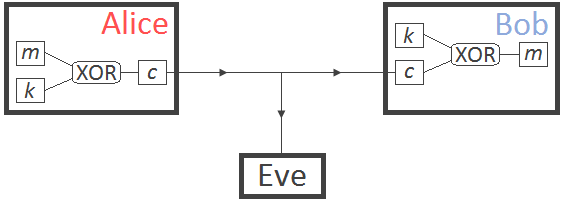
\includegraphics{images/one-time_pad.png}

The one-time pad method is proved to be be absolutely secure. Thus, if
Eve intercepted the ciphertext \(c\), she will not get any information
from the message \(m\) until she has the key \(k\).

The main problem of modern cryptographic systems is the distribution
among the participants of the communication session of a secret key,
possession of which should not be available to third parties. The
rapidly developing methods of quantum key distribution can solve this
problem regardless of the capabilities of the eavesdropper. In this
tutorial, we show how Alice and Bob can generate a secret key using the
\emph{E91} quantum key distribution protocol.

    \subsection{\texorpdfstring{\emph{Quantum
entanglement}}{Quantum entanglement}}\label{quantum-entanglement}

    The E91 protocol developed by Artur Ekert in 1991 is based on the use of
entangled states and Bell's theorem (see
\href{https://github.com/QISKit/qiskit-tutorial/blob/master/2_quantum_information/entanglement_revisited.ipynb}{Entanglement
Revisited} QISKit tutorial). It is known that two electrons \emph{A} and
\emph{B} can be prepared in such a state that they can not be considered
separately from each other. One of these states is the singlet state

\[\lvert\psi_s\rangle =
  \frac{1}{\sqrt{2}}(\lvert0\rangle_A\otimes\lvert1\rangle_B - \lvert1\rangle_A\otimes\lvert0\rangle_B) =
  \frac{1}{\sqrt{2}}(\lvert01\rangle - \lvert10\rangle),\]

where the vectors \(\lvert 0 \rangle\) and \(\lvert 1 \rangle\) describe
the states of each electron with the
{[}spin{]}(https://en.wikipedia.org/wiki/Spin\_(physics\%29) projection
along the positive and negative direction of the \emph{z} axis.

The observable of the projection of the spin onto the direction
\(\vec{n}=(n_x, n_y, n_z)\) is given by

\[\vec{n} \cdot \vec{\sigma} = 
n_x X + n_y Y + n_z Z,\]

where \(\vec{\sigma} = (X, Y, Z)\) and \(X, Y, Z\) are the Pauli
matrices. For two qubits \emph{A} and \emph{B}, the observable
\((\vec{a} \cdot \vec{\sigma})_A \otimes (\vec{b} \cdot \vec{\sigma})_B\)
describes the joint measurement of the spin projections onto the
directions \(\vec{a}\) and \(\vec{b}\). It can be shown that the
expectation value of this observable in the singlet state is

\[\langle (\vec{a} \cdot \vec{\sigma})_A \otimes (\vec{b} \cdot \vec{\sigma})_B \rangle_{\psi_s} =
-\vec{a} \cdot \vec{b}. \qquad\qquad (1)\]

Here we see an interesting fact: if Alice and Bob measure the spin
projections of electrons A and B onto the same direction, they will
obtain the opposite results. Thus, if Alice got the result \(\pm 1\),
then Bob \emph{definitely} will get the result \(\mp 1\), i.e. the
results will be perfectly anticorrelated.

    \subsection{\texorpdfstring{\emph{CHSH
inequality}}{CHSH inequality}}\label{chsh-inequality}

    In the framework of classical physics, it is impossible to create a
correlation inherent in the singlet state \(\lvert\psi_s\rangle\).
Indeed, let us measure the observables \(X\), \(Z\) for qubit \emph{A}
and observables \(W = \frac{1}{\sqrt{2}} (X + Z)\),
\(V = \frac{1}{\sqrt{2}} (-X + Z)\) for qubit \emph{B}. Performing joint
measurements of these observables, the following expectation values can
be obtained:

\begin{eqnarray*}
 \langle X \otimes W \rangle_{\psi_s} &= -\frac{1}{\sqrt{2}}, \quad 
 \langle X \otimes V \rangle_{\psi_s} &= \frac{1}{\sqrt{2}}, \qquad\qquad (2) \\
 \langle Z \otimes W \rangle_{\psi_s} &= -\frac{1}{\sqrt{2}}, \quad
 \langle Z \otimes V \rangle_{\psi_s} &= -\frac{1}{\sqrt{2}}.
\end{eqnarray*}

Now we can costruct the \emph{Clauser-Horne-Shimony-Holt (CHSH)
correlation value}:

\[C =
\langle X\otimes W \rangle - \langle X \otimes V \rangle + \langle Z \otimes W \rangle + \langle Z \otimes V \rangle =
-2 \sqrt{2}. \qquad\qquad (3)\]

The
\href{https://en.wikipedia.org/wiki/Local_hidden_variable_theory}{local
hidden variable theory} which was developed in particular to explain the
quantum correlations gives that \(\lvert C \rvert \leqslant 2\). But
\href{https://en.wikipedia.org/wiki/Bell's_theorem}{Bell's theorem}
states that "no physical theory of local hidden variables can ever
reproduce all of the predictions of quantum mechanics." Thus, the
violation of the
\href{https://en.wikipedia.org/wiki/Bell's_theorem\#Bell_inequalities_are_violated_by_quantum_mechanical_predictions}{CHSH
inequality} (i.e. \(C = -2 \sqrt{2}\) for the singlet state), which is a
generalized form of Bell's inequality, can serve as an \emph{indicator
of quantum entanglement}. This fact finds its application in the E91
protocol.

    \subsection{\texorpdfstring{\emph{The
protocol}}{The protocol}}\label{the-protocol}

To implement the E91 quantum key distribution protocol, there must be a
source of qubits prepared in the singlet state. It does not matter to
whom this source belongs: to Alice, to Bob, to some trusted third-party
Charlie or even to Eve.

The steps of the E91 protocol are following.

    \begin{enumerate}
\def\labelenumi{\arabic{enumi}.}
\item
  Charlie, the owner of the singlet state preparation device, creates
  \(N\) entangled states \(\lvert\psi_s\rangle\) and sends qubits
  \emph{A} to Alice and qubits \emph{B} to Bob via the quantum channel.
  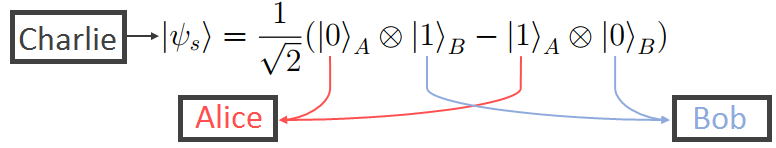
\includegraphics{images/singlet_distribution.png}
\item
  Participants Alice and Bob generate strings \(b=(b_1 \ldots b_N)\) and
  \(b^{'}=(b_1^{'} \ldots b_N^{'})\), where \(b_i, b^{'}_j = 1, 2, 3\).
  Depending on the elements of these strings, Alice and Bob measure the
  spin projections of their qubits along the following directions:

  \begin{align*}
   b_i = 1: \quad \vec{a}_1 &= (1,0,0) \quad (X \text{ observable}) &
   b_j^{'} = 1: \quad \vec{b}_1 &= \left(\frac{1}{\sqrt{2}},0,\frac{1}{\sqrt{2}}\right) \quad (W \text{ observable})
   \\
   b_i = 2: \quad \vec{a}_2 &= \left(\frac{1}{\sqrt{2}},0,\frac{1}{\sqrt{2}}\right) \quad (W \text{ observable}) &
   b_j^{'} = 2: \quad \vec{b}_2 &= (0,0,1) \quad ( \text{Z observable})
   \\
   b_i = 3: \quad \vec{a}_3 &= (0,0,1) \quad (Z \text{ observable}) &
   b_j^{'} = 3: \quad \vec{b}_3 &= \left(-\frac{1}{\sqrt{2}},0,\frac{1}{\sqrt{2}}\right) \quad (V \text{ observable})
  \end{align*}

   Trusted Notebook" width="500 px" align="center"\textgreater{} We can
  describe this process as a measurement of the observables
  \((\vec{a}_i \cdot \vec{\sigma})_A \otimes (\vec{b}_j \cdot \vec{\sigma})_B\)
  for each singlet state created by Charlie.
\item
  Alice and Bob record the results of their measurements as elements of
  strings \(a=(a_1 \ldots a_N)\) and \(a^{'} =(a_1^{'} \ldots a_N^{'})\)
  respectively, where \(a_i, a^{'}_j = \pm 1\).
\item
  Using the classical channel, participants compare their strings
  \(b=(b_1 \ldots b_N)\) and \(b^{'}=(b_1^{'} \ldots b_N^{'})\). In
  other words, Alice and Bob tell each other which measurements they
  have performed during the step 2. If Alice and Bob have measured the
  spin projections of the \(m\)-th entangled pair of qubits onto the
  same direction (i.e. \(\vec{a}_2/\vec{b}_1\) or
  \(\vec{a}_3/\vec{b}_2\) for Alice's and Bob's qubit respectively),
  then they are sure that they obtained opposite results, i.e.
  \(a_m = - a_m^{'}\) (see Eq. (1)). Thus, for the \(l\)-th bit of the
  key strings \(k=(k_1 \ldots k_n),k^{'}=(k_1^{'} \ldots k_n^{'})\)
  Alice and Bob can write \(k_l = a_m, k_l^{'} = -a_m^{'}\).
  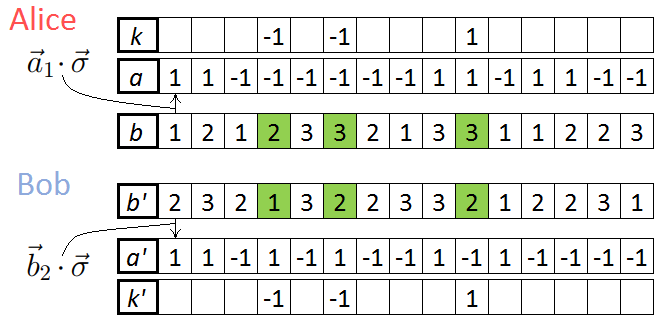
\includegraphics{images/step3-4strings.png}
\item
  Using the results obtained after measuring the spin projections onto
  the \(\vec{a}_1/\vec{b}_1\), \(\vec{a}_1/\vec{b}_3\),
  \(\vec{a}_3/\vec{b}_1\) and \(\vec{a}_3/\vec{b}_3\) directions
  (observables \((2)\)), Alice and Bob calculate the CHSH correlation
  value \((3)\). If \(C = -2\sqrt{2}\), then Alice and Bob can be sure
  that the states they had been receiving from Charlie were entangled
  indeed. This fact tells the participants that there was no
  interference in the quantum channel.
\end{enumerate}

    \subsection{\texorpdfstring{\emph{Simulation}}{Simulation}}\label{simulation}

In this section we simulate the E91 quantum key distribution protocol
\emph{without} the presence of an eavesdropper.

    \subsubsection{\texorpdfstring{\emph{Step one: creating the
singlets}}{Step one: creating the singlets}}\label{step-one-creating-the-singlets}

In the first step Alice and Bob receive their qubits of the singlet
states \(\lvert\psi_s\rangle\) created by Charlie.

For our simulation, we need registers with two quantum bits and four
classical bits.

    \begin{Verbatim}[commandchars=\\\{\}]
{\color{incolor}In [{\color{incolor}1}]:} \PY{c+c1}{\PYZsh{} Checking the version of PYTHON; we only support \PYZgt{} 3.5}
        \PY{k+kn}{import} \PY{n+nn}{sys}
        \PY{k}{if} \PY{n}{sys}\PY{o}{.}\PY{n}{version\PYZus{}info} \PY{o}{\PYZlt{}} \PY{p}{(}\PY{l+m+mi}{3}\PY{p}{,}\PY{l+m+mi}{5}\PY{p}{)}\PY{p}{:}
            \PY{k}{raise} \PY{n+ne}{Exception}\PY{p}{(}\PY{l+s+s1}{\PYZsq{}}\PY{l+s+s1}{Please use Python version 3.5 or greater.}\PY{l+s+s1}{\PYZsq{}}\PY{p}{)}
            
        \PY{c+c1}{\PYZsh{} useful additional packages }
        \PY{k+kn}{import} \PY{n+nn}{numpy} \PY{k}{as} \PY{n+nn}{np}
        \PY{k+kn}{import} \PY{n+nn}{random}
        \PY{k+kn}{import} \PY{n+nn}{math}
        \PY{k+kn}{import} \PY{n+nn}{re} \PY{c+c1}{\PYZsh{} regular expressions module}
        
        \PY{c+c1}{\PYZsh{} importing the QISKit}
        \PY{k+kn}{from} \PY{n+nn}{qiskit} \PY{k}{import} \PY{n}{QuantumCircuit}\PY{p}{,} \PY{n}{QuantumProgram}
        \PY{k+kn}{import} \PY{n+nn}{Qconfig}
        
        \PY{c+c1}{\PYZsh{} Quantum program setup}
        \PY{n}{Q\PYZus{}program} \PY{o}{=} \PY{n}{QuantumProgram}\PY{p}{(}\PY{p}{)}
        \PY{c+c1}{\PYZsh{}Q\PYZus{}program.set\PYZus{}api(Qconfig.APItoken, Qconfig.config[\PYZsq{}url\PYZsq{}]) \PYZsh{} set the APIToken and API url}
        
        \PY{c+c1}{\PYZsh{} Creating registers}
        \PY{n}{qr} \PY{o}{=} \PY{n}{Q\PYZus{}program}\PY{o}{.}\PY{n}{create\PYZus{}quantum\PYZus{}register}\PY{p}{(}\PY{l+s+s2}{\PYZdq{}}\PY{l+s+s2}{qr}\PY{l+s+s2}{\PYZdq{}}\PY{p}{,} \PY{l+m+mi}{2}\PY{p}{)}
        \PY{n}{cr} \PY{o}{=} \PY{n}{Q\PYZus{}program}\PY{o}{.}\PY{n}{create\PYZus{}classical\PYZus{}register}\PY{p}{(}\PY{l+s+s2}{\PYZdq{}}\PY{l+s+s2}{cr}\PY{l+s+s2}{\PYZdq{}}\PY{p}{,} \PY{l+m+mi}{4}\PY{p}{)}
\end{Verbatim}


    \begin{Verbatim}[commandchars=\\\{\}]
WARNING:qiskit.\_util:Could not find IBMQuantumExperience in requirements.txt or the requirements.txt                 file was not found or unparsable

    \end{Verbatim}

    Let us assume that qubits \emph{qr{[}0{]}} and \emph{qr{[}1{]}} belong
to Alice and Bob respetively. In classical bits \emph{cr{[}0{]}} and
\emph{cr{[}1{]}} Alice and Bob store their measurement results, and
classical bits \emph{cr{[}2{]}} and \emph{cr{[}3{]}} are used by Eve to
store her measurement results of Alice's and Bob's qubits.

Now Charlie creates a singlet state:

    \begin{Verbatim}[commandchars=\\\{\}]
{\color{incolor}In [{\color{incolor}2}]:} \PY{n}{singlet} \PY{o}{=} \PY{n}{Q\PYZus{}program}\PY{o}{.}\PY{n}{create\PYZus{}circuit}\PY{p}{(}\PY{l+s+s1}{\PYZsq{}}\PY{l+s+s1}{singlet}\PY{l+s+s1}{\PYZsq{}}\PY{p}{,} \PY{p}{[}\PY{n}{qr}\PY{p}{]}\PY{p}{,} \PY{p}{[}\PY{n}{cr}\PY{p}{]}\PY{p}{)}
        \PY{n}{singlet}\PY{o}{.}\PY{n}{x}\PY{p}{(}\PY{n}{qr}\PY{p}{[}\PY{l+m+mi}{0}\PY{p}{]}\PY{p}{)}
        \PY{n}{singlet}\PY{o}{.}\PY{n}{x}\PY{p}{(}\PY{n}{qr}\PY{p}{[}\PY{l+m+mi}{1}\PY{p}{]}\PY{p}{)}
        \PY{n}{singlet}\PY{o}{.}\PY{n}{h}\PY{p}{(}\PY{n}{qr}\PY{p}{[}\PY{l+m+mi}{0}\PY{p}{]}\PY{p}{)}
        \PY{n}{singlet}\PY{o}{.}\PY{n}{cx}\PY{p}{(}\PY{n}{qr}\PY{p}{[}\PY{l+m+mi}{0}\PY{p}{]}\PY{p}{,}\PY{n}{qr}\PY{p}{[}\PY{l+m+mi}{1}\PY{p}{]}\PY{p}{)}
\end{Verbatim}


\begin{Verbatim}[commandchars=\\\{\}]
{\color{outcolor}Out[{\color{outcolor}2}]:} <qiskit.extensions.standard.cx.CnotGate at 0xebdf4cc8d0>
\end{Verbatim}
            
    Qubits \emph{qr{[}0{]}} and \emph{qr{[}1{]}} are now entangled. After
creating a singlet state, Charlie sends qubit \emph{qr{[}0{]}} to Alice
and qubit \emph{qr{[}1{]}} to Bob.
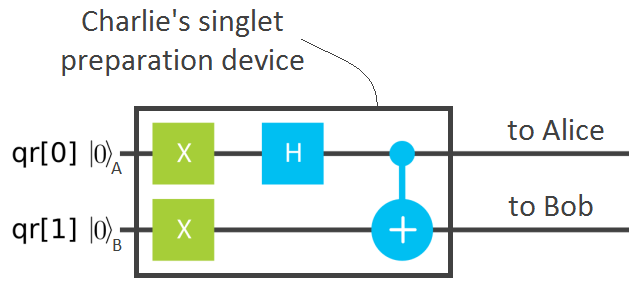
\includegraphics{images/singlet_device.png}

    \subsubsection{\texorpdfstring{\emph{Step two:
measuring}}{Step two: measuring}}\label{step-two-measuring}

    First let us prepare the measurements which will be used by Alice and
Bob. We define \(A(\vec{a}_i) = \vec{a}_i \cdot \vec{\sigma}\) and
\(B(\vec{b}_j) = \vec{b}_j \cdot \vec{\sigma}\) as the spin projection
observables used by Alice and Bob for their measurements. To perform
these measurements, the standard basis \(Z\) must be rotated to the
proper basis when it is needed (see
\href{https://quantumexperience.ng.bluemix.net/proxy/tutorial/full-user-guide/002-The_Weird_and_Wonderful_World_of_the_Qubit/020-Superposition.html}{Superposition}
and
\href{https://quantumexperience.ng.bluemix.net/proxy/tutorial/full-user-guide/003-Multiple_Qubits_Gates_and_Entangled_States/050-Entanglement_and_Bell_Tests.html}{Entanglement
and Bell Tests} user guides). Here we define the notation of possible
measurements of Alice and Bob: 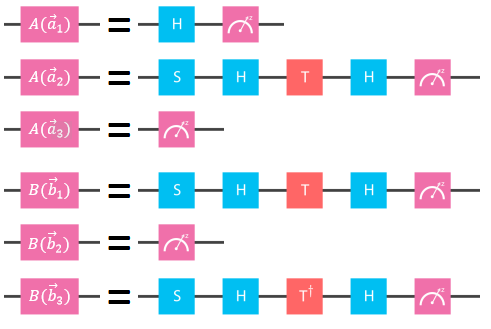
\includegraphics{images/bases.png}

    Blocks on the left side can be considered as \emph{detectors} used by
the participants to measure \(X, W, Z\) and \(V\) observables. Now we
prepare the corresponding curcuits.

    \begin{Verbatim}[commandchars=\\\{\}]
{\color{incolor}In [{\color{incolor}3}]:} \PY{c+c1}{\PYZsh{}\PYZsh{} Alice\PYZsq{}s measurement circuits}
        
        \PY{c+c1}{\PYZsh{} measure the spin projection of Alice\PYZsq{}s qubit onto the a\PYZus{}1 direction (X basis)}
        \PY{n}{measureA1} \PY{o}{=} \PY{n}{Q\PYZus{}program}\PY{o}{.}\PY{n}{create\PYZus{}circuit}\PY{p}{(}\PY{l+s+s1}{\PYZsq{}}\PY{l+s+s1}{measureA1}\PY{l+s+s1}{\PYZsq{}}\PY{p}{,} \PY{p}{[}\PY{n}{qr}\PY{p}{]}\PY{p}{,} \PY{p}{[}\PY{n}{cr}\PY{p}{]}\PY{p}{)}
        \PY{n}{measureA1}\PY{o}{.}\PY{n}{h}\PY{p}{(}\PY{n}{qr}\PY{p}{[}\PY{l+m+mi}{0}\PY{p}{]}\PY{p}{)}
        \PY{n}{measureA1}\PY{o}{.}\PY{n}{measure}\PY{p}{(}\PY{n}{qr}\PY{p}{[}\PY{l+m+mi}{0}\PY{p}{]}\PY{p}{,}\PY{n}{cr}\PY{p}{[}\PY{l+m+mi}{0}\PY{p}{]}\PY{p}{)}
        
        \PY{c+c1}{\PYZsh{} measure the spin projection of Alice\PYZsq{}s qubit onto the a\PYZus{}2 direction (W basis)}
        \PY{n}{measureA2} \PY{o}{=} \PY{n}{Q\PYZus{}program}\PY{o}{.}\PY{n}{create\PYZus{}circuit}\PY{p}{(}\PY{l+s+s1}{\PYZsq{}}\PY{l+s+s1}{measureA2}\PY{l+s+s1}{\PYZsq{}}\PY{p}{,} \PY{p}{[}\PY{n}{qr}\PY{p}{]}\PY{p}{,} \PY{p}{[}\PY{n}{cr}\PY{p}{]}\PY{p}{)}
        \PY{n}{measureA2}\PY{o}{.}\PY{n}{s}\PY{p}{(}\PY{n}{qr}\PY{p}{[}\PY{l+m+mi}{0}\PY{p}{]}\PY{p}{)}
        \PY{n}{measureA2}\PY{o}{.}\PY{n}{h}\PY{p}{(}\PY{n}{qr}\PY{p}{[}\PY{l+m+mi}{0}\PY{p}{]}\PY{p}{)}
        \PY{n}{measureA2}\PY{o}{.}\PY{n}{t}\PY{p}{(}\PY{n}{qr}\PY{p}{[}\PY{l+m+mi}{0}\PY{p}{]}\PY{p}{)}
        \PY{n}{measureA2}\PY{o}{.}\PY{n}{h}\PY{p}{(}\PY{n}{qr}\PY{p}{[}\PY{l+m+mi}{0}\PY{p}{]}\PY{p}{)}
        \PY{n}{measureA2}\PY{o}{.}\PY{n}{measure}\PY{p}{(}\PY{n}{qr}\PY{p}{[}\PY{l+m+mi}{0}\PY{p}{]}\PY{p}{,}\PY{n}{cr}\PY{p}{[}\PY{l+m+mi}{0}\PY{p}{]}\PY{p}{)}
        
        \PY{c+c1}{\PYZsh{} measure the spin projection of Alice\PYZsq{}s qubit onto the a\PYZus{}3 direction (standard Z basis)}
        \PY{n}{measureA3} \PY{o}{=} \PY{n}{Q\PYZus{}program}\PY{o}{.}\PY{n}{create\PYZus{}circuit}\PY{p}{(}\PY{l+s+s1}{\PYZsq{}}\PY{l+s+s1}{measureA3}\PY{l+s+s1}{\PYZsq{}}\PY{p}{,} \PY{p}{[}\PY{n}{qr}\PY{p}{]}\PY{p}{,} \PY{p}{[}\PY{n}{cr}\PY{p}{]}\PY{p}{)}
        \PY{n}{measureA3}\PY{o}{.}\PY{n}{measure}\PY{p}{(}\PY{n}{qr}\PY{p}{[}\PY{l+m+mi}{0}\PY{p}{]}\PY{p}{,}\PY{n}{cr}\PY{p}{[}\PY{l+m+mi}{0}\PY{p}{]}\PY{p}{)}
        
        \PY{c+c1}{\PYZsh{}\PYZsh{} Bob\PYZsq{}s measurement circuits}
        
        \PY{c+c1}{\PYZsh{} measure the spin projection of Bob\PYZsq{}s qubit onto the b\PYZus{}1 direction (W basis)}
        \PY{n}{measureB1} \PY{o}{=} \PY{n}{Q\PYZus{}program}\PY{o}{.}\PY{n}{create\PYZus{}circuit}\PY{p}{(}\PY{l+s+s1}{\PYZsq{}}\PY{l+s+s1}{measureB1}\PY{l+s+s1}{\PYZsq{}}\PY{p}{,} \PY{p}{[}\PY{n}{qr}\PY{p}{]}\PY{p}{,} \PY{p}{[}\PY{n}{cr}\PY{p}{]}\PY{p}{)}
        \PY{n}{measureB1}\PY{o}{.}\PY{n}{s}\PY{p}{(}\PY{n}{qr}\PY{p}{[}\PY{l+m+mi}{1}\PY{p}{]}\PY{p}{)}
        \PY{n}{measureB1}\PY{o}{.}\PY{n}{h}\PY{p}{(}\PY{n}{qr}\PY{p}{[}\PY{l+m+mi}{1}\PY{p}{]}\PY{p}{)}
        \PY{n}{measureB1}\PY{o}{.}\PY{n}{t}\PY{p}{(}\PY{n}{qr}\PY{p}{[}\PY{l+m+mi}{1}\PY{p}{]}\PY{p}{)}
        \PY{n}{measureB1}\PY{o}{.}\PY{n}{h}\PY{p}{(}\PY{n}{qr}\PY{p}{[}\PY{l+m+mi}{1}\PY{p}{]}\PY{p}{)}
        \PY{n}{measureB1}\PY{o}{.}\PY{n}{measure}\PY{p}{(}\PY{n}{qr}\PY{p}{[}\PY{l+m+mi}{1}\PY{p}{]}\PY{p}{,}\PY{n}{cr}\PY{p}{[}\PY{l+m+mi}{1}\PY{p}{]}\PY{p}{)}
        
        \PY{c+c1}{\PYZsh{} measure the spin projection of Bob\PYZsq{}s qubit onto the b\PYZus{}2 direction (standard Z basis)}
        \PY{n}{measureB2} \PY{o}{=} \PY{n}{Q\PYZus{}program}\PY{o}{.}\PY{n}{create\PYZus{}circuit}\PY{p}{(}\PY{l+s+s1}{\PYZsq{}}\PY{l+s+s1}{measureB2}\PY{l+s+s1}{\PYZsq{}}\PY{p}{,} \PY{p}{[}\PY{n}{qr}\PY{p}{]}\PY{p}{,} \PY{p}{[}\PY{n}{cr}\PY{p}{]}\PY{p}{)}
        \PY{n}{measureB2}\PY{o}{.}\PY{n}{measure}\PY{p}{(}\PY{n}{qr}\PY{p}{[}\PY{l+m+mi}{1}\PY{p}{]}\PY{p}{,}\PY{n}{cr}\PY{p}{[}\PY{l+m+mi}{1}\PY{p}{]}\PY{p}{)}
        
        \PY{c+c1}{\PYZsh{} measure the spin projection of Bob\PYZsq{}s qubit onto the b\PYZus{}3 direction (V basis)}
        \PY{n}{measureB3} \PY{o}{=} \PY{n}{Q\PYZus{}program}\PY{o}{.}\PY{n}{create\PYZus{}circuit}\PY{p}{(}\PY{l+s+s1}{\PYZsq{}}\PY{l+s+s1}{measureB3}\PY{l+s+s1}{\PYZsq{}}\PY{p}{,} \PY{p}{[}\PY{n}{qr}\PY{p}{]}\PY{p}{,} \PY{p}{[}\PY{n}{cr}\PY{p}{]}\PY{p}{)}
        \PY{n}{measureB3}\PY{o}{.}\PY{n}{s}\PY{p}{(}\PY{n}{qr}\PY{p}{[}\PY{l+m+mi}{1}\PY{p}{]}\PY{p}{)}
        \PY{n}{measureB3}\PY{o}{.}\PY{n}{h}\PY{p}{(}\PY{n}{qr}\PY{p}{[}\PY{l+m+mi}{1}\PY{p}{]}\PY{p}{)}
        \PY{n}{measureB3}\PY{o}{.}\PY{n}{tdg}\PY{p}{(}\PY{n}{qr}\PY{p}{[}\PY{l+m+mi}{1}\PY{p}{]}\PY{p}{)}
        \PY{n}{measureB3}\PY{o}{.}\PY{n}{h}\PY{p}{(}\PY{n}{qr}\PY{p}{[}\PY{l+m+mi}{1}\PY{p}{]}\PY{p}{)}
        \PY{n}{measureB3}\PY{o}{.}\PY{n}{measure}\PY{p}{(}\PY{n}{qr}\PY{p}{[}\PY{l+m+mi}{1}\PY{p}{]}\PY{p}{,}\PY{n}{cr}\PY{p}{[}\PY{l+m+mi}{1}\PY{p}{]}\PY{p}{)}
        
        \PY{c+c1}{\PYZsh{}\PYZsh{} Lists of measurement circuits}
        \PY{n}{aliceMeasurements} \PY{o}{=} \PY{p}{[}\PY{n}{measureA1}\PY{p}{,} \PY{n}{measureA2}\PY{p}{,} \PY{n}{measureA3}\PY{p}{]}
        \PY{n}{bobMeasurements} \PY{o}{=} \PY{p}{[}\PY{n}{measureB1}\PY{p}{,} \PY{n}{measureB2}\PY{p}{,} \PY{n}{measureB3}\PY{p}{]}
\end{Verbatim}


    Supose Alice and Bob want to generate a secret key using \(N\) singlet
states prepared by Charlie.

    \begin{Verbatim}[commandchars=\\\{\}]
{\color{incolor}In [{\color{incolor}4}]:} \PY{c+c1}{\PYZsh{} Define the number of singlets N}
        \PY{n}{numberOfSinglets} \PY{o}{=} \PY{l+m+mi}{500}
\end{Verbatim}


    The participants must choose the directions onto which they will measure
the spin projections of their qubits. To do this, Alice and Bob create
the strings \(b\) and \(b^{'}\) with randomly generated elements.

    \begin{Verbatim}[commandchars=\\\{\}]
{\color{incolor}In [{\color{incolor}5}]:} \PY{n}{aliceMeasurementChoices} \PY{o}{=} \PY{p}{[}\PY{n}{random}\PY{o}{.}\PY{n}{randint}\PY{p}{(}\PY{l+m+mi}{1}\PY{p}{,} \PY{l+m+mi}{3}\PY{p}{)} \PY{k}{for} \PY{n}{i} \PY{o+ow}{in} \PY{n+nb}{range}\PY{p}{(}\PY{n}{numberOfSinglets}\PY{p}{)}\PY{p}{]} \PY{c+c1}{\PYZsh{} string b of Alice}
        \PY{n}{bobMeasurementChoices} \PY{o}{=} \PY{p}{[}\PY{n}{random}\PY{o}{.}\PY{n}{randint}\PY{p}{(}\PY{l+m+mi}{1}\PY{p}{,} \PY{l+m+mi}{3}\PY{p}{)} \PY{k}{for} \PY{n}{i} \PY{o+ow}{in} \PY{n+nb}{range}\PY{p}{(}\PY{n}{numberOfSinglets}\PY{p}{)}\PY{p}{]} \PY{c+c1}{\PYZsh{} string b\PYZsq{} of Bob}
\end{Verbatim}


    Now we combine Charlie's device and Alice's and Bob's detectors into one
circuit (singlet + Alice's measurement + Bob's measurement).

    \begin{Verbatim}[commandchars=\\\{\}]
{\color{incolor}In [{\color{incolor}6}]:} \PY{n}{circuits} \PY{o}{=} \PY{p}{[}\PY{p}{]} \PY{c+c1}{\PYZsh{} the list in which the created circuits will be stored}
        
        \PY{k}{for} \PY{n}{i} \PY{o+ow}{in} \PY{n+nb}{range}\PY{p}{(}\PY{n}{numberOfSinglets}\PY{p}{)}\PY{p}{:}
            \PY{c+c1}{\PYZsh{} create the name of the i\PYZhy{}th circuit depending on Alice\PYZsq{}s and Bob\PYZsq{}s measurement choices}
            \PY{n}{circuitName} \PY{o}{=} \PY{n+nb}{str}\PY{p}{(}\PY{n}{i}\PY{p}{)} \PY{o}{+} \PY{l+s+s1}{\PYZsq{}}\PY{l+s+s1}{:A}\PY{l+s+s1}{\PYZsq{}} \PY{o}{+} \PY{n+nb}{str}\PY{p}{(}\PY{n}{aliceMeasurementChoices}\PY{p}{[}\PY{n}{i}\PY{p}{]}\PY{p}{)} \PY{o}{+} \PY{l+s+s1}{\PYZsq{}}\PY{l+s+s1}{\PYZus{}B}\PY{l+s+s1}{\PYZsq{}} \PY{o}{+} \PY{n+nb}{str}\PY{p}{(}\PY{n}{bobMeasurementChoices}\PY{p}{[}\PY{n}{i}\PY{p}{]}\PY{p}{)}
            
            \PY{c+c1}{\PYZsh{} create the joint measurement circuit}
            \PY{c+c1}{\PYZsh{} add Alice\PYZsq{}s and Bob\PYZsq{}s measurement circuits to the singlet state curcuit}
            \PY{n}{Q\PYZus{}program}\PY{o}{.}\PY{n}{add\PYZus{}circuit}\PY{p}{(}\PY{n}{circuitName}\PY{p}{,}
                                  \PY{n}{singlet} \PY{o}{+} \PY{c+c1}{\PYZsh{} singlet state circuit}
                                  \PY{n}{aliceMeasurements}\PY{p}{[}\PY{n}{aliceMeasurementChoices}\PY{p}{[}\PY{n}{i}\PY{p}{]}\PY{o}{\PYZhy{}}\PY{l+m+mi}{1}\PY{p}{]} \PY{o}{+} \PY{c+c1}{\PYZsh{} measurement circuit of Alice}
                                  \PY{n}{bobMeasurements}\PY{p}{[}\PY{n}{bobMeasurementChoices}\PY{p}{[}\PY{n}{i}\PY{p}{]}\PY{o}{\PYZhy{}}\PY{l+m+mi}{1}\PY{p}{]} \PY{c+c1}{\PYZsh{} measurement circuit of Bob}
                                 \PY{p}{)}
            
            \PY{c+c1}{\PYZsh{} add the created circuit to the circuits list}
            \PY{n}{circuits}\PY{o}{.}\PY{n}{append}\PY{p}{(}\PY{n}{circuitName}\PY{p}{)}
\end{Verbatim}


    Let us look at the name of one of the prepared circuits.

    \begin{Verbatim}[commandchars=\\\{\}]
{\color{incolor}In [{\color{incolor}7}]:} \PY{n+nb}{print}\PY{p}{(}\PY{n}{circuits}\PY{p}{[}\PY{l+m+mi}{0}\PY{p}{]}\PY{p}{)}
\end{Verbatim}


    \begin{Verbatim}[commandchars=\\\{\}]
0:A1\_B2

    \end{Verbatim}

    It tells us about the number of the singlet state received from Charlie,
and the measurements applied by Alice and Bob.

In the \emph{circuits} list we have stored \(N\)
(\emph{numberOfSinglets}) circuits similar to those shown in the figure
below. 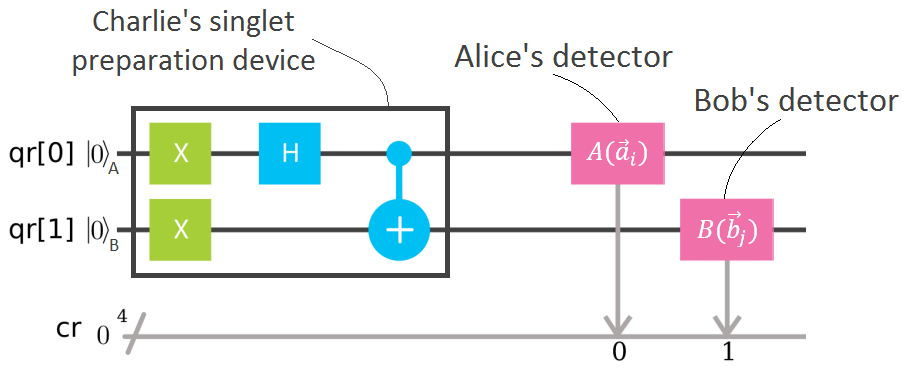
\includegraphics{images/AB_circuit.png}

The idea is to model every act of the creation of the singlet state, the
distribution of its qubits among the participants and the measurement of
the spin projection onto the chosen direction in the E91 protocol by
executing each circuit from the \emph{circuits} list with one shot.

    \subsubsection{\texorpdfstring{\emph{Step three: recording the
results}}{Step three: recording the results}}\label{step-three-recording-the-results}

    First let us execute the circuits on the simulator.

    \begin{Verbatim}[commandchars=\\\{\}]
{\color{incolor}In [{\color{incolor}8}]:} \PY{n}{result} \PY{o}{=} \PY{n}{Q\PYZus{}program}\PY{o}{.}\PY{n}{execute}\PY{p}{(}\PY{n}{circuits}\PY{p}{,} \PY{n}{backend}\PY{o}{=}\PY{l+s+s1}{\PYZsq{}}\PY{l+s+s1}{local\PYZus{}qasm\PYZus{}simulator}\PY{l+s+s1}{\PYZsq{}}\PY{p}{,} \PY{n}{shots}\PY{o}{=}\PY{l+m+mi}{1}\PY{p}{,} \PY{n}{max\PYZus{}credits}\PY{o}{=}\PY{l+m+mi}{5}\PY{p}{,} \PY{n}{wait}\PY{o}{=}\PY{l+m+mi}{10}\PY{p}{,} \PY{n}{timeout}\PY{o}{=}\PY{l+m+mi}{240}\PY{p}{)}
        \PY{n+nb}{print}\PY{p}{(}\PY{n}{result}\PY{p}{)}
\end{Verbatim}


    \begin{Verbatim}[commandchars=\\\{\}]
COMPLETED

    \end{Verbatim}

    Look at the output of the execution of the first circuit.

    \begin{Verbatim}[commandchars=\\\{\}]
{\color{incolor}In [{\color{incolor}9}]:} \PY{n}{result}\PY{o}{.}\PY{n}{get\PYZus{}counts}\PY{p}{(}\PY{n}{circuits}\PY{p}{[}\PY{l+m+mi}{0}\PY{p}{]}\PY{p}{)}
\end{Verbatim}


\begin{Verbatim}[commandchars=\\\{\}]
{\color{outcolor}Out[{\color{outcolor}9}]:} \{'0001': 1\}
\end{Verbatim}
            
    It consists of four digits. Recall that Alice and Bob store the results
of the measurement in classical bits \emph{cr{[}0{]}} and
\emph{cr{[}1{]}} (two digits on the right). Since we model the secret
key generation process without the presence of an eavesdropper, the
classical bits \emph{cr{[}2{]}} and \emph{cr{[}3{]}} are always 0. Also
note that the output is the Python dictionary, in which the keys are the
obtained results, and the values are the counts.

Alice and Bob record the results of their measurements as bits of the
strings \(a\) and \(a^{'}\). To simulate this process we need to use
regular expressions module
\emph{\href{https://docs.python.org/3/howto/regex.html\#regex-howto}{re}}.
First, we compile the search patterns.

    \begin{Verbatim}[commandchars=\\\{\}]
{\color{incolor}In [{\color{incolor}10}]:} \PY{n}{abPatterns} \PY{o}{=} \PY{p}{[}
             \PY{n}{re}\PY{o}{.}\PY{n}{compile}\PY{p}{(}\PY{l+s+s1}{\PYZsq{}}\PY{l+s+s1}{..00\PYZdl{}}\PY{l+s+s1}{\PYZsq{}}\PY{p}{)}\PY{p}{,} \PY{c+c1}{\PYZsh{} search for the \PYZsq{}..00\PYZsq{} output (Alice obtained \PYZhy{}1 and Bob obtained \PYZhy{}1)}
             \PY{n}{re}\PY{o}{.}\PY{n}{compile}\PY{p}{(}\PY{l+s+s1}{\PYZsq{}}\PY{l+s+s1}{..01\PYZdl{}}\PY{l+s+s1}{\PYZsq{}}\PY{p}{)}\PY{p}{,} \PY{c+c1}{\PYZsh{} search for the \PYZsq{}..01\PYZsq{} output}
             \PY{n}{re}\PY{o}{.}\PY{n}{compile}\PY{p}{(}\PY{l+s+s1}{\PYZsq{}}\PY{l+s+s1}{..10\PYZdl{}}\PY{l+s+s1}{\PYZsq{}}\PY{p}{)}\PY{p}{,} \PY{c+c1}{\PYZsh{} search for the \PYZsq{}..10\PYZsq{} output (Alice obtained \PYZhy{}1 and Bob obtained 1)}
             \PY{n}{re}\PY{o}{.}\PY{n}{compile}\PY{p}{(}\PY{l+s+s1}{\PYZsq{}}\PY{l+s+s1}{..11\PYZdl{}}\PY{l+s+s1}{\PYZsq{}}\PY{p}{)}  \PY{c+c1}{\PYZsh{} search for the \PYZsq{}..11\PYZsq{} output}
         \PY{p}{]}
\end{Verbatim}


    Using these patterns, we can find particular results in the outputs and
fill strings the \(a\) and \(a^{'}\) with the results of Alice's and
Bob's measurements.

    \begin{Verbatim}[commandchars=\\\{\}]
{\color{incolor}In [{\color{incolor}11}]:} \PY{n}{aliceResults} \PY{o}{=} \PY{p}{[}\PY{p}{]} \PY{c+c1}{\PYZsh{} Alice\PYZsq{}s results (string a)}
         \PY{n}{bobResults} \PY{o}{=} \PY{p}{[}\PY{p}{]} \PY{c+c1}{\PYZsh{} Bob\PYZsq{}s results (string a\PYZsq{})}
         
         \PY{k}{for} \PY{n}{i} \PY{o+ow}{in} \PY{n+nb}{range}\PY{p}{(}\PY{n}{numberOfSinglets}\PY{p}{)}\PY{p}{:}
         
             \PY{n}{res} \PY{o}{=} \PY{n+nb}{list}\PY{p}{(}\PY{n}{result}\PY{o}{.}\PY{n}{get\PYZus{}counts}\PY{p}{(}\PY{n}{circuits}\PY{p}{[}\PY{n}{i}\PY{p}{]}\PY{p}{)}\PY{o}{.}\PY{n}{keys}\PY{p}{(}\PY{p}{)}\PY{p}{)}\PY{p}{[}\PY{l+m+mi}{0}\PY{p}{]} \PY{c+c1}{\PYZsh{} extract the key from the dict and transform it to str; execution result of the i\PYZhy{}th circuit}
             
             \PY{k}{if} \PY{n}{abPatterns}\PY{p}{[}\PY{l+m+mi}{0}\PY{p}{]}\PY{o}{.}\PY{n}{search}\PY{p}{(}\PY{n}{res}\PY{p}{)}\PY{p}{:} \PY{c+c1}{\PYZsh{} check if the key is \PYZsq{}..00\PYZsq{} (if the measurement results are \PYZhy{}1,\PYZhy{}1)}
                 \PY{n}{aliceResults}\PY{o}{.}\PY{n}{append}\PY{p}{(}\PY{o}{\PYZhy{}}\PY{l+m+mi}{1}\PY{p}{)} \PY{c+c1}{\PYZsh{} Alice got the result \PYZhy{}1 }
                 \PY{n}{bobResults}\PY{o}{.}\PY{n}{append}\PY{p}{(}\PY{o}{\PYZhy{}}\PY{l+m+mi}{1}\PY{p}{)} \PY{c+c1}{\PYZsh{} Bob got the result \PYZhy{}1}
             \PY{k}{if} \PY{n}{abPatterns}\PY{p}{[}\PY{l+m+mi}{1}\PY{p}{]}\PY{o}{.}\PY{n}{search}\PY{p}{(}\PY{n}{res}\PY{p}{)}\PY{p}{:}
                 \PY{n}{aliceResults}\PY{o}{.}\PY{n}{append}\PY{p}{(}\PY{l+m+mi}{1}\PY{p}{)}
                 \PY{n}{bobResults}\PY{o}{.}\PY{n}{append}\PY{p}{(}\PY{o}{\PYZhy{}}\PY{l+m+mi}{1}\PY{p}{)}
             \PY{k}{if} \PY{n}{abPatterns}\PY{p}{[}\PY{l+m+mi}{2}\PY{p}{]}\PY{o}{.}\PY{n}{search}\PY{p}{(}\PY{n}{res}\PY{p}{)}\PY{p}{:} \PY{c+c1}{\PYZsh{} check if the key is \PYZsq{}..10\PYZsq{} (if the measurement results are \PYZhy{}1,1)}
                 \PY{n}{aliceResults}\PY{o}{.}\PY{n}{append}\PY{p}{(}\PY{o}{\PYZhy{}}\PY{l+m+mi}{1}\PY{p}{)} \PY{c+c1}{\PYZsh{} Alice got the result \PYZhy{}1 }
                 \PY{n}{bobResults}\PY{o}{.}\PY{n}{append}\PY{p}{(}\PY{l+m+mi}{1}\PY{p}{)} \PY{c+c1}{\PYZsh{} Bob got the result 1}
             \PY{k}{if} \PY{n}{abPatterns}\PY{p}{[}\PY{l+m+mi}{3}\PY{p}{]}\PY{o}{.}\PY{n}{search}\PY{p}{(}\PY{n}{res}\PY{p}{)}\PY{p}{:} 
                 \PY{n}{aliceResults}\PY{o}{.}\PY{n}{append}\PY{p}{(}\PY{l+m+mi}{1}\PY{p}{)}
                 \PY{n}{bobResults}\PY{o}{.}\PY{n}{append}\PY{p}{(}\PY{l+m+mi}{1}\PY{p}{)}
\end{Verbatim}


    \subsubsection{\texorpdfstring{\emph{Step four: revealing the
bases}}{Step four: revealing the bases}}\label{step-four-revealing-the-bases}

    In the previos step we have stored the measurement results of Alice and
Bob in the \emph{aliceResults} and \emph{bobResults} lists (strings
\(a\) and \(a^{'}\)). Now the participants compare their strings \(b\)
and \(b^{'}\) via the public classical channel. If Alice and Bob have
measured the spin projections of their qubits of the \emph{i}-th singlet
onto the same direction, then Alice records the result \(a_i\) as the
bit of the string \(k\), and Bob records the result \(-a_i\) as the bit
of the string \(k^{'}\) (see Eq. (1)).

    \begin{Verbatim}[commandchars=\\\{\}]
{\color{incolor}In [{\color{incolor}12}]:} \PY{n}{aliceKey} \PY{o}{=} \PY{p}{[}\PY{p}{]} \PY{c+c1}{\PYZsh{} Alice\PYZsq{}s key string k}
         \PY{n}{bobKey} \PY{o}{=} \PY{p}{[}\PY{p}{]} \PY{c+c1}{\PYZsh{} Bob\PYZsq{}s key string k\PYZsq{}}
         
         \PY{c+c1}{\PYZsh{} comparing the stings with measurement choices}
         \PY{k}{for} \PY{n}{i} \PY{o+ow}{in} \PY{n+nb}{range}\PY{p}{(}\PY{n}{numberOfSinglets}\PY{p}{)}\PY{p}{:}
             \PY{c+c1}{\PYZsh{} if Alice and Bob have measured the spin projections onto the a\PYZus{}2/b\PYZus{}1 or a\PYZus{}3/b\PYZus{}2 directions}
             \PY{k}{if} \PY{p}{(}\PY{n}{aliceMeasurementChoices}\PY{p}{[}\PY{n}{i}\PY{p}{]} \PY{o}{==} \PY{l+m+mi}{2} \PY{o+ow}{and} \PY{n}{bobMeasurementChoices}\PY{p}{[}\PY{n}{i}\PY{p}{]} \PY{o}{==} \PY{l+m+mi}{1}\PY{p}{)} \PY{o+ow}{or} \PY{p}{(}\PY{n}{aliceMeasurementChoices}\PY{p}{[}\PY{n}{i}\PY{p}{]} \PY{o}{==} \PY{l+m+mi}{3} \PY{o+ow}{and} \PY{n}{bobMeasurementChoices}\PY{p}{[}\PY{n}{i}\PY{p}{]} \PY{o}{==} \PY{l+m+mi}{2}\PY{p}{)}\PY{p}{:}
                 \PY{n}{aliceKey}\PY{o}{.}\PY{n}{append}\PY{p}{(}\PY{n}{aliceResults}\PY{p}{[}\PY{n}{i}\PY{p}{]}\PY{p}{)} \PY{c+c1}{\PYZsh{} record the i\PYZhy{}th result obtained by Alice as the bit of the secret key k}
                 \PY{n}{bobKey}\PY{o}{.}\PY{n}{append}\PY{p}{(}\PY{o}{\PYZhy{}} \PY{n}{bobResults}\PY{p}{[}\PY{n}{i}\PY{p}{]}\PY{p}{)} \PY{c+c1}{\PYZsh{} record the multiplied by \PYZhy{}1 i\PYZhy{}th result obtained Bob as the bit of the secret key k\PYZsq{}}
                 
         \PY{n}{keyLength} \PY{o}{=} \PY{n+nb}{len}\PY{p}{(}\PY{n}{aliceKey}\PY{p}{)} \PY{c+c1}{\PYZsh{} length of the secret key}
\end{Verbatim}


    The keys \(k\) and \(k'\) are now stored in the \emph{aliceKey} and
\emph{bobKey} lists, respectively. The remaining results which were not
used to create the keys can now be revealed.

It is important for Alice and Bob to have the same keys, i.e. strings
\(k\) and \(k^{'}\) must be equal. Let us compare the bits of strings
\(k\) and \(k^{'}\) and find out how many there are mismatches in the
keys.

    \begin{Verbatim}[commandchars=\\\{\}]
{\color{incolor}In [{\color{incolor}13}]:} \PY{n}{abKeyMismatches} \PY{o}{=} \PY{l+m+mi}{0} \PY{c+c1}{\PYZsh{} number of mismatching bits in Alice\PYZsq{}s and Bob\PYZsq{}s keys}
         
         \PY{k}{for} \PY{n}{j} \PY{o+ow}{in} \PY{n+nb}{range}\PY{p}{(}\PY{n}{keyLength}\PY{p}{)}\PY{p}{:}
             \PY{k}{if} \PY{n}{aliceKey}\PY{p}{[}\PY{n}{j}\PY{p}{]} \PY{o}{!=} \PY{n}{bobKey}\PY{p}{[}\PY{n}{j}\PY{p}{]}\PY{p}{:}
                 \PY{n}{abKeyMismatches} \PY{o}{+}\PY{o}{=} \PY{l+m+mi}{1}
\end{Verbatim}


    Note that since the strings \(k\) and \(k^{'}\) are secret, Alice and
Bob have no information about mismatches in the bits of their keys. To
find out the number of errors, the participants can perform a random
sampling test. Alice randomly selects \(\delta\) bits of her secret key
and tells Bob which bits she selected. Then Alice and Bob compare the
values of these check bits. For large enough \(\delta\) the number of
errors in the check bits will be close to the number of errors in the
remaining bits.

    \subsubsection{\texorpdfstring{\emph{Step five: CHSH correlation value
test}}{Step five: CHSH correlation value test}}\label{step-five-chsh-correlation-value-test}

    Alice and Bob want to be sure that there was no interference in the
communication session. To do that, they calculate the CHSH correlation
value \((3)\) using the results obtained after the measurements of spin
projections onto the \(\vec{a}_1/\vec{b}_1\), \(\vec{a}_1/\vec{b}_3\),
\(\vec{a}_3/\vec{b}_1\) and \(\vec{a}_3/\vec{b}_3\) directions. Recall
that it is equivalent to the measurement of the observables
\(X \otimes W\), \(X \otimes V\), \(Z \otimes W\) and \(Z \otimes V\)
respectively.

According to the Born-von Neumann statistical postulate, the expectation
value of the observable
\(E = \sum_j e_j \lvert e_j \rangle \langle e_j \rvert\) in the state
\(\lvert \psi \rangle\) is given by

\[\langle E \rangle_\psi =
  \mathrm{Tr}\, \lvert\psi\rangle \langle\psi\rvert \, E = \\
  \mathrm{Tr}\, \lvert\psi\rangle \langle\psi\rvert \sum_j e_j \lvert e_j \rangle \langle e_j \rvert  = 
  \sum_j \langle\psi\rvert(e_j \lvert e_j \rangle \langle e_j \rvert) \lvert\psi\rangle = 
  \sum_j e_j \left|\langle\psi\lvert e_j \rangle \right|^2 = \\
  \sum_j e_j \mathrm{P}_\psi (E \models e_j),\] where
\(\lvert e_j \rangle\) is the eigenvector of \(E\) with the
corresponding eigenvalue \(e_j\), and
\(\mathrm{P}_\psi (E \models e_j)\) is the probability of obtainig the
result \(e_j\) after measuring the observable \(E\) in the state
\(\lvert \psi \rangle\).

A similar expression can be written for the joint measurement of the
observables \(A\) and \(B\):

\[\langle A \otimes B \rangle_\psi =
  \sum_{j,k} a_j b_k \mathrm{P}_\psi (A \models a_j, B \models b_k) =
  \sum_{j,k} a_j b_k \mathrm{P}_\psi (a_j, b_k). \qquad\qquad (4)\]

Note that if \(A\) and \(B\) are the spin projection observables, then
the corresponding eigenvalues are \(a_j, b_k = \pm 1\). Thus, for the
observables \(A(\vec{a}_i)\) and \(B(\vec{b}_j)\) and singlet state
\(\lvert\psi\rangle_s\) we can rewrite \((4)\) as

\[\langle A(\vec{a}_i) \otimes B(\vec{b}_j) \rangle =
  \mathrm{P}(-1,-1) - \mathrm{P}(1,-1) - \mathrm{P}(-1,1) + \mathrm{P}(1,1). \qquad\qquad (5)\]

In our experiments, the probabilities on the right side can be
calculated as follows:

\[\mathrm{P}(a_j, b_k) = \frac{n_{a_j, b_k}(A \otimes B)}{N(A \otimes B)}, \qquad\qquad (6)\]

where the numerator is the number of results \(a_j, b_k\) obtained after
measuring the observable \(A \otimes B\), and the denominator is the
total number of measurements of the observable \(A \otimes B\).

Since Alice and Bob revealed their strings \(b\) and \(b^{'}\), they
know what measurements they performed and what results they have
obtained. With this data, participants calculate the expectation values
\((2)\) using \((5)\) and \((6)\).

    \begin{Verbatim}[commandchars=\\\{\}]
{\color{incolor}In [{\color{incolor}14}]:} \PY{c+c1}{\PYZsh{} function that calculates CHSH correlation value}
         \PY{k}{def} \PY{n+nf}{chsh\PYZus{}corr}\PY{p}{(}\PY{n}{result}\PY{p}{)}\PY{p}{:}
             
             \PY{c+c1}{\PYZsh{} lists with the counts of measurement results}
             \PY{c+c1}{\PYZsh{} each element represents the number of (\PYZhy{}1,\PYZhy{}1), (\PYZhy{}1,1), (1,\PYZhy{}1) and (1,1) results respectively}
             \PY{n}{countA1B1} \PY{o}{=} \PY{p}{[}\PY{l+m+mi}{0}\PY{p}{,} \PY{l+m+mi}{0}\PY{p}{,} \PY{l+m+mi}{0}\PY{p}{,} \PY{l+m+mi}{0}\PY{p}{]} \PY{c+c1}{\PYZsh{} XW observable}
             \PY{n}{countA1B3} \PY{o}{=} \PY{p}{[}\PY{l+m+mi}{0}\PY{p}{,} \PY{l+m+mi}{0}\PY{p}{,} \PY{l+m+mi}{0}\PY{p}{,} \PY{l+m+mi}{0}\PY{p}{]} \PY{c+c1}{\PYZsh{} XV observable}
             \PY{n}{countA3B1} \PY{o}{=} \PY{p}{[}\PY{l+m+mi}{0}\PY{p}{,} \PY{l+m+mi}{0}\PY{p}{,} \PY{l+m+mi}{0}\PY{p}{,} \PY{l+m+mi}{0}\PY{p}{]} \PY{c+c1}{\PYZsh{} ZW observable}
             \PY{n}{countA3B3} \PY{o}{=} \PY{p}{[}\PY{l+m+mi}{0}\PY{p}{,} \PY{l+m+mi}{0}\PY{p}{,} \PY{l+m+mi}{0}\PY{p}{,} \PY{l+m+mi}{0}\PY{p}{]} \PY{c+c1}{\PYZsh{} ZV observable}
         
             \PY{k}{for} \PY{n}{i} \PY{o+ow}{in} \PY{n+nb}{range}\PY{p}{(}\PY{n}{numberOfSinglets}\PY{p}{)}\PY{p}{:}
         
                 \PY{n}{res} \PY{o}{=} \PY{n+nb}{list}\PY{p}{(}\PY{n}{result}\PY{o}{.}\PY{n}{get\PYZus{}counts}\PY{p}{(}\PY{n}{circuits}\PY{p}{[}\PY{n}{i}\PY{p}{]}\PY{p}{)}\PY{o}{.}\PY{n}{keys}\PY{p}{(}\PY{p}{)}\PY{p}{)}\PY{p}{[}\PY{l+m+mi}{0}\PY{p}{]}
         
                 \PY{c+c1}{\PYZsh{} if the spins of the qubits of the i\PYZhy{}th singlet were projected onto the a\PYZus{}1/b\PYZus{}1 directions}
                 \PY{k}{if} \PY{p}{(}\PY{n}{aliceMeasurementChoices}\PY{p}{[}\PY{n}{i}\PY{p}{]} \PY{o}{==} \PY{l+m+mi}{1} \PY{o+ow}{and} \PY{n}{bobMeasurementChoices}\PY{p}{[}\PY{n}{i}\PY{p}{]} \PY{o}{==} \PY{l+m+mi}{1}\PY{p}{)}\PY{p}{:}
                     \PY{k}{for} \PY{n}{j} \PY{o+ow}{in} \PY{n+nb}{range}\PY{p}{(}\PY{l+m+mi}{4}\PY{p}{)}\PY{p}{:}
                         \PY{k}{if} \PY{n}{abPatterns}\PY{p}{[}\PY{n}{j}\PY{p}{]}\PY{o}{.}\PY{n}{search}\PY{p}{(}\PY{n}{res}\PY{p}{)}\PY{p}{:}
                             \PY{n}{countA1B1}\PY{p}{[}\PY{n}{j}\PY{p}{]} \PY{o}{+}\PY{o}{=} \PY{l+m+mi}{1}
         
                 \PY{k}{if} \PY{p}{(}\PY{n}{aliceMeasurementChoices}\PY{p}{[}\PY{n}{i}\PY{p}{]} \PY{o}{==} \PY{l+m+mi}{1} \PY{o+ow}{and} \PY{n}{bobMeasurementChoices}\PY{p}{[}\PY{n}{i}\PY{p}{]} \PY{o}{==} \PY{l+m+mi}{3}\PY{p}{)}\PY{p}{:}
                     \PY{k}{for} \PY{n}{j} \PY{o+ow}{in} \PY{n+nb}{range}\PY{p}{(}\PY{l+m+mi}{4}\PY{p}{)}\PY{p}{:}
                         \PY{k}{if} \PY{n}{abPatterns}\PY{p}{[}\PY{n}{j}\PY{p}{]}\PY{o}{.}\PY{n}{search}\PY{p}{(}\PY{n}{res}\PY{p}{)}\PY{p}{:}
                             \PY{n}{countA1B3}\PY{p}{[}\PY{n}{j}\PY{p}{]} \PY{o}{+}\PY{o}{=} \PY{l+m+mi}{1}
         
                 \PY{k}{if} \PY{p}{(}\PY{n}{aliceMeasurementChoices}\PY{p}{[}\PY{n}{i}\PY{p}{]} \PY{o}{==} \PY{l+m+mi}{3} \PY{o+ow}{and} \PY{n}{bobMeasurementChoices}\PY{p}{[}\PY{n}{i}\PY{p}{]} \PY{o}{==} \PY{l+m+mi}{1}\PY{p}{)}\PY{p}{:}
                     \PY{k}{for} \PY{n}{j} \PY{o+ow}{in} \PY{n+nb}{range}\PY{p}{(}\PY{l+m+mi}{4}\PY{p}{)}\PY{p}{:}
                         \PY{k}{if} \PY{n}{abPatterns}\PY{p}{[}\PY{n}{j}\PY{p}{]}\PY{o}{.}\PY{n}{search}\PY{p}{(}\PY{n}{res}\PY{p}{)}\PY{p}{:}
                             \PY{n}{countA3B1}\PY{p}{[}\PY{n}{j}\PY{p}{]} \PY{o}{+}\PY{o}{=} \PY{l+m+mi}{1}
                             
                 \PY{c+c1}{\PYZsh{} if the spins of the qubits of the i\PYZhy{}th singlet were projected onto the a\PYZus{}3/b\PYZus{}3 directions}
                 \PY{k}{if} \PY{p}{(}\PY{n}{aliceMeasurementChoices}\PY{p}{[}\PY{n}{i}\PY{p}{]} \PY{o}{==} \PY{l+m+mi}{3} \PY{o+ow}{and} \PY{n}{bobMeasurementChoices}\PY{p}{[}\PY{n}{i}\PY{p}{]} \PY{o}{==} \PY{l+m+mi}{3}\PY{p}{)}\PY{p}{:}
                     \PY{k}{for} \PY{n}{j} \PY{o+ow}{in} \PY{n+nb}{range}\PY{p}{(}\PY{l+m+mi}{4}\PY{p}{)}\PY{p}{:}
                         \PY{k}{if} \PY{n}{abPatterns}\PY{p}{[}\PY{n}{j}\PY{p}{]}\PY{o}{.}\PY{n}{search}\PY{p}{(}\PY{n}{res}\PY{p}{)}\PY{p}{:}
                             \PY{n}{countA3B3}\PY{p}{[}\PY{n}{j}\PY{p}{]} \PY{o}{+}\PY{o}{=} \PY{l+m+mi}{1}
                             
             \PY{c+c1}{\PYZsh{} number of the results obtained from the measurements in a particular basis}
             \PY{n}{total11} \PY{o}{=} \PY{n+nb}{sum}\PY{p}{(}\PY{n}{countA1B1}\PY{p}{)}
             \PY{n}{total13} \PY{o}{=} \PY{n+nb}{sum}\PY{p}{(}\PY{n}{countA1B3}\PY{p}{)}
             \PY{n}{total31} \PY{o}{=} \PY{n+nb}{sum}\PY{p}{(}\PY{n}{countA3B1}\PY{p}{)}
             \PY{n}{total33} \PY{o}{=} \PY{n+nb}{sum}\PY{p}{(}\PY{n}{countA3B3}\PY{p}{)}      
                             
             \PY{c+c1}{\PYZsh{} expectation values of XW, XV, ZW and ZV observables (2)}
             \PY{n}{expect11} \PY{o}{=} \PY{p}{(}\PY{n}{countA1B1}\PY{p}{[}\PY{l+m+mi}{0}\PY{p}{]} \PY{o}{\PYZhy{}} \PY{n}{countA1B1}\PY{p}{[}\PY{l+m+mi}{1}\PY{p}{]} \PY{o}{\PYZhy{}} \PY{n}{countA1B1}\PY{p}{[}\PY{l+m+mi}{2}\PY{p}{]} \PY{o}{+} \PY{n}{countA1B1}\PY{p}{[}\PY{l+m+mi}{3}\PY{p}{]}\PY{p}{)}\PY{o}{/}\PY{n}{total11} \PY{c+c1}{\PYZsh{} \PYZhy{}1/sqrt(2)}
             \PY{n}{expect13} \PY{o}{=} \PY{p}{(}\PY{n}{countA1B3}\PY{p}{[}\PY{l+m+mi}{0}\PY{p}{]} \PY{o}{\PYZhy{}} \PY{n}{countA1B3}\PY{p}{[}\PY{l+m+mi}{1}\PY{p}{]} \PY{o}{\PYZhy{}} \PY{n}{countA1B3}\PY{p}{[}\PY{l+m+mi}{2}\PY{p}{]} \PY{o}{+} \PY{n}{countA1B3}\PY{p}{[}\PY{l+m+mi}{3}\PY{p}{]}\PY{p}{)}\PY{o}{/}\PY{n}{total13} \PY{c+c1}{\PYZsh{} 1/sqrt(2)}
             \PY{n}{expect31} \PY{o}{=} \PY{p}{(}\PY{n}{countA3B1}\PY{p}{[}\PY{l+m+mi}{0}\PY{p}{]} \PY{o}{\PYZhy{}} \PY{n}{countA3B1}\PY{p}{[}\PY{l+m+mi}{1}\PY{p}{]} \PY{o}{\PYZhy{}} \PY{n}{countA3B1}\PY{p}{[}\PY{l+m+mi}{2}\PY{p}{]} \PY{o}{+} \PY{n}{countA3B1}\PY{p}{[}\PY{l+m+mi}{3}\PY{p}{]}\PY{p}{)}\PY{o}{/}\PY{n}{total31} \PY{c+c1}{\PYZsh{} \PYZhy{}1/sqrt(2)}
             \PY{n}{expect33} \PY{o}{=} \PY{p}{(}\PY{n}{countA3B3}\PY{p}{[}\PY{l+m+mi}{0}\PY{p}{]} \PY{o}{\PYZhy{}} \PY{n}{countA3B3}\PY{p}{[}\PY{l+m+mi}{1}\PY{p}{]} \PY{o}{\PYZhy{}} \PY{n}{countA3B3}\PY{p}{[}\PY{l+m+mi}{2}\PY{p}{]} \PY{o}{+} \PY{n}{countA3B3}\PY{p}{[}\PY{l+m+mi}{3}\PY{p}{]}\PY{p}{)}\PY{o}{/}\PY{n}{total33} \PY{c+c1}{\PYZsh{} \PYZhy{}1/sqrt(2) }
             
             \PY{n}{corr} \PY{o}{=} \PY{n}{expect11} \PY{o}{\PYZhy{}} \PY{n}{expect13} \PY{o}{+} \PY{n}{expect31} \PY{o}{+} \PY{n}{expect33} \PY{c+c1}{\PYZsh{} calculate the CHSC correlation value (3)}
             
             \PY{k}{return} \PY{n}{corr}
\end{Verbatim}


    \subsubsection{\texorpdfstring{\emph{Output}}{Output}}\label{output}

    Now let us print all the interesting values.

    \begin{Verbatim}[commandchars=\\\{\}]
{\color{incolor}In [{\color{incolor}15}]:} \PY{n}{corr} \PY{o}{=} \PY{n}{chsh\PYZus{}corr}\PY{p}{(}\PY{n}{result}\PY{p}{)} \PY{c+c1}{\PYZsh{} CHSH correlation value}
         
         \PY{c+c1}{\PYZsh{} CHSH inequality test}
         \PY{n+nb}{print}\PY{p}{(}\PY{l+s+s1}{\PYZsq{}}\PY{l+s+s1}{CHSH correlation value: }\PY{l+s+s1}{\PYZsq{}} \PY{o}{+} \PY{n+nb}{str}\PY{p}{(}\PY{n+nb}{round}\PY{p}{(}\PY{n}{corr}\PY{p}{,} \PY{l+m+mi}{3}\PY{p}{)}\PY{p}{)}\PY{p}{)}
         
         \PY{c+c1}{\PYZsh{} Keys}
         \PY{n+nb}{print}\PY{p}{(}\PY{l+s+s1}{\PYZsq{}}\PY{l+s+s1}{Length of the key: }\PY{l+s+s1}{\PYZsq{}} \PY{o}{+} \PY{n+nb}{str}\PY{p}{(}\PY{n}{keyLength}\PY{p}{)}\PY{p}{)}
         \PY{n+nb}{print}\PY{p}{(}\PY{l+s+s1}{\PYZsq{}}\PY{l+s+s1}{Number of mismatching bits: }\PY{l+s+s1}{\PYZsq{}} \PY{o}{+} \PY{n+nb}{str}\PY{p}{(}\PY{n}{abKeyMismatches}\PY{p}{)} \PY{o}{+} \PY{l+s+s1}{\PYZsq{}}\PY{l+s+se}{\PYZbs{}n}\PY{l+s+s1}{\PYZsq{}}\PY{p}{)}
\end{Verbatim}


    \begin{Verbatim}[commandchars=\\\{\}]
CHSH correlation value: -2.954
Length of the key: 120
Number of mismatching bits: 0


    \end{Verbatim}

    Finaly, Alice and Bob have the secret keys \(k\) and \(k^{'}\)
(\emph{aliceKey} and \emph{bobKey})! Now they can use the one-time pad
technique to encrypt and decrypt messages.

Since we simulate the E91 protocol without the presence of Eve, the CHSH
correlation value should be close to \(-2\sqrt{2} \approx -2.828\). In
addition, there should be no mismatching bits in the keys of Alice and
Bob. Note also that there are 9 possible combinations of measurements
that can be performed by Alice and Bob, but only 2 of them give the
results using which the secret keys can be created. Thus, the ratio of
the length of the keys to the number of singlets \(N\) should be close
to \(2/9\).

    \subsection{\texorpdfstring{\emph{Simulation of
eavesdropping}}{Simulation of eavesdropping}}\label{simulation-of-eavesdropping}

    Suppose some third party wants to interfere in the communication session
of Alice and Bob and obtain a secret key. The eavesdropper can use the
\emph{intercept-resend} attacks: Eve intercepts one or both of the
entangled qubits prepared by Charlie, measures the spin projections of
these qubits, prepares new ones depending on the results obtained
(\(\lvert 01 \rangle\) or \(\lvert 10 \rangle\)) and sends them to Alice
and Bob. A schematic representation of this process is shown in the
figure below. 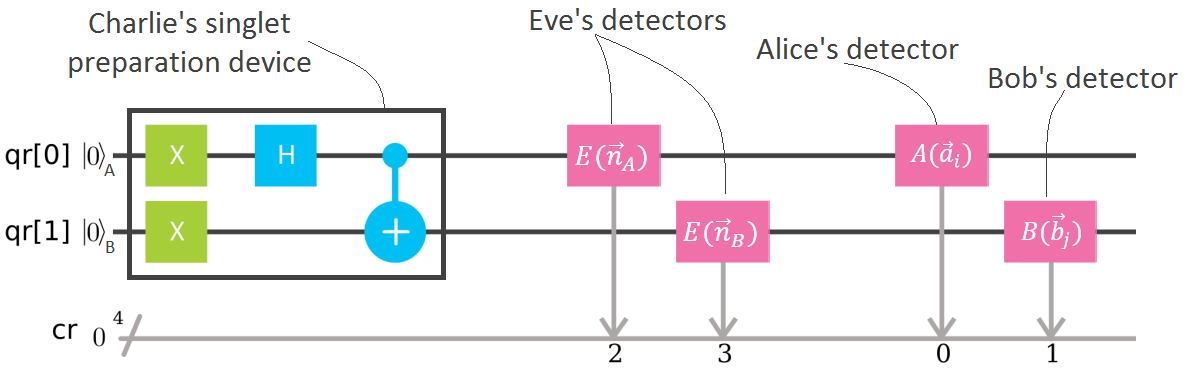
\includegraphics{images/ABE_circuit.png}

Here \(E(\vec{n}_A) = \vec{n}_A \cdot \vec{\sigma}\) and
\(E(\vec{n}_B) = \vec{n}_A \cdot \vec{\sigma}\) are the observables of
the of the spin projections of Alice's and Bob's qubits onto the
directions \(\vec{n}_A\) and \(\vec{n}_B\). It would be wise for Eve to
choose these directions to be \(\vec{n}_A = \vec{a}_2,\vec{a}_3\) and
\(\vec{n}_B = \vec{b}_1,\vec{b}_2\) since the results obtained from
other measurements can not be used to create a secret key.

Let us prepare the circuits for Eve's measurements.

    \begin{Verbatim}[commandchars=\\\{\}]
{\color{incolor}In [{\color{incolor}16}]:} \PY{c+c1}{\PYZsh{} measurement of the spin projection of Alice\PYZsq{}s qubit onto the a\PYZus{}2 direction (W basis)}
         \PY{n}{measureEA2} \PY{o}{=} \PY{n}{Q\PYZus{}program}\PY{o}{.}\PY{n}{create\PYZus{}circuit}\PY{p}{(}\PY{l+s+s1}{\PYZsq{}}\PY{l+s+s1}{measureEA2}\PY{l+s+s1}{\PYZsq{}}\PY{p}{,} \PY{p}{[}\PY{n}{qr}\PY{p}{]}\PY{p}{,} \PY{p}{[}\PY{n}{cr}\PY{p}{]}\PY{p}{)}
         \PY{n}{measureEA2}\PY{o}{.}\PY{n}{s}\PY{p}{(}\PY{n}{qr}\PY{p}{[}\PY{l+m+mi}{0}\PY{p}{]}\PY{p}{)}
         \PY{n}{measureEA2}\PY{o}{.}\PY{n}{h}\PY{p}{(}\PY{n}{qr}\PY{p}{[}\PY{l+m+mi}{0}\PY{p}{]}\PY{p}{)}
         \PY{n}{measureEA2}\PY{o}{.}\PY{n}{t}\PY{p}{(}\PY{n}{qr}\PY{p}{[}\PY{l+m+mi}{0}\PY{p}{]}\PY{p}{)}
         \PY{n}{measureEA2}\PY{o}{.}\PY{n}{h}\PY{p}{(}\PY{n}{qr}\PY{p}{[}\PY{l+m+mi}{0}\PY{p}{]}\PY{p}{)}
         \PY{n}{measureEA2}\PY{o}{.}\PY{n}{measure}\PY{p}{(}\PY{n}{qr}\PY{p}{[}\PY{l+m+mi}{0}\PY{p}{]}\PY{p}{,}\PY{n}{cr}\PY{p}{[}\PY{l+m+mi}{2}\PY{p}{]}\PY{p}{)}
         
         \PY{c+c1}{\PYZsh{} measurement of the spin projection of Allice\PYZsq{}s qubit onto the a\PYZus{}3 direction (standard Z basis)}
         \PY{n}{measureEA3} \PY{o}{=} \PY{n}{Q\PYZus{}program}\PY{o}{.}\PY{n}{create\PYZus{}circuit}\PY{p}{(}\PY{l+s+s1}{\PYZsq{}}\PY{l+s+s1}{measureEA3}\PY{l+s+s1}{\PYZsq{}}\PY{p}{,} \PY{p}{[}\PY{n}{qr}\PY{p}{]}\PY{p}{,} \PY{p}{[}\PY{n}{cr}\PY{p}{]}\PY{p}{)}
         \PY{n}{measureEA3}\PY{o}{.}\PY{n}{measure}\PY{p}{(}\PY{n}{qr}\PY{p}{[}\PY{l+m+mi}{0}\PY{p}{]}\PY{p}{,}\PY{n}{cr}\PY{p}{[}\PY{l+m+mi}{2}\PY{p}{]}\PY{p}{)}
         
         \PY{c+c1}{\PYZsh{} measurement of the spin projection of Bob\PYZsq{}s qubit onto the b\PYZus{}1 direction (W basis)}
         \PY{n}{measureEB1} \PY{o}{=} \PY{n}{Q\PYZus{}program}\PY{o}{.}\PY{n}{create\PYZus{}circuit}\PY{p}{(}\PY{l+s+s1}{\PYZsq{}}\PY{l+s+s1}{measureEB1}\PY{l+s+s1}{\PYZsq{}}\PY{p}{,} \PY{p}{[}\PY{n}{qr}\PY{p}{]}\PY{p}{,} \PY{p}{[}\PY{n}{cr}\PY{p}{]}\PY{p}{)}
         \PY{n}{measureEB1}\PY{o}{.}\PY{n}{s}\PY{p}{(}\PY{n}{qr}\PY{p}{[}\PY{l+m+mi}{1}\PY{p}{]}\PY{p}{)}
         \PY{n}{measureEB1}\PY{o}{.}\PY{n}{h}\PY{p}{(}\PY{n}{qr}\PY{p}{[}\PY{l+m+mi}{1}\PY{p}{]}\PY{p}{)}
         \PY{n}{measureEB1}\PY{o}{.}\PY{n}{t}\PY{p}{(}\PY{n}{qr}\PY{p}{[}\PY{l+m+mi}{1}\PY{p}{]}\PY{p}{)}
         \PY{n}{measureEB1}\PY{o}{.}\PY{n}{h}\PY{p}{(}\PY{n}{qr}\PY{p}{[}\PY{l+m+mi}{1}\PY{p}{]}\PY{p}{)}
         \PY{n}{measureEB1}\PY{o}{.}\PY{n}{measure}\PY{p}{(}\PY{n}{qr}\PY{p}{[}\PY{l+m+mi}{1}\PY{p}{]}\PY{p}{,}\PY{n}{cr}\PY{p}{[}\PY{l+m+mi}{3}\PY{p}{]}\PY{p}{)}
         
         \PY{c+c1}{\PYZsh{} measurement of the spin projection of Bob\PYZsq{}s qubit onto the b\PYZus{}2 direction (standard Z measurement)}
         \PY{n}{measureEB2} \PY{o}{=} \PY{n}{Q\PYZus{}program}\PY{o}{.}\PY{n}{create\PYZus{}circuit}\PY{p}{(}\PY{l+s+s1}{\PYZsq{}}\PY{l+s+s1}{measureEB2}\PY{l+s+s1}{\PYZsq{}}\PY{p}{,} \PY{p}{[}\PY{n}{qr}\PY{p}{]}\PY{p}{,} \PY{p}{[}\PY{n}{cr}\PY{p}{]}\PY{p}{)}
         \PY{n}{measureEB2}\PY{o}{.}\PY{n}{measure}\PY{p}{(}\PY{n}{qr}\PY{p}{[}\PY{l+m+mi}{1}\PY{p}{]}\PY{p}{,}\PY{n}{cr}\PY{p}{[}\PY{l+m+mi}{3}\PY{p}{]}\PY{p}{)}
         
         \PY{c+c1}{\PYZsh{} lists of measurement circuits}
         \PY{n}{eveMeasurements} \PY{o}{=} \PY{p}{[}\PY{n}{measureEA2}\PY{p}{,} \PY{n}{measureEA3}\PY{p}{,} \PY{n}{measureEB1}\PY{p}{,} \PY{n}{measureEB2}\PY{p}{]}
\end{Verbatim}


    Like Alice and Bob, Eve must choose the directions onto which she will
measure the spin projections of the qubits. In our simulation, the
eavesdropper randomly chooses one of the observables \(W \otimes W\) or
\(Z \otimes Z\) to measure.

    \begin{Verbatim}[commandchars=\\\{\}]
{\color{incolor}In [{\color{incolor}17}]:} \PY{c+c1}{\PYZsh{} list of Eve\PYZsq{}s measurement choices}
         \PY{c+c1}{\PYZsh{} the first and the second elements of each row represent the measurement of Alice\PYZsq{}s and Bob\PYZsq{}s qubits by Eve respectively}
         \PY{n}{eveMeasurementChoices} \PY{o}{=} \PY{p}{[}\PY{p}{]}
         
         \PY{k}{for} \PY{n}{j} \PY{o+ow}{in} \PY{n+nb}{range}\PY{p}{(}\PY{n}{numberOfSinglets}\PY{p}{)}\PY{p}{:}      
             \PY{k}{if} \PY{n}{random}\PY{o}{.}\PY{n}{uniform}\PY{p}{(}\PY{l+m+mi}{0}\PY{p}{,} \PY{l+m+mi}{1}\PY{p}{)} \PY{o}{\PYZlt{}}\PY{o}{=} \PY{l+m+mf}{0.5}\PY{p}{:} \PY{c+c1}{\PYZsh{} in 50\PYZpc{} of cases perform the WW measurement}
                 \PY{n}{eveMeasurementChoices}\PY{o}{.}\PY{n}{append}\PY{p}{(}\PY{p}{[}\PY{l+m+mi}{0}\PY{p}{,} \PY{l+m+mi}{2}\PY{p}{]}\PY{p}{)}
             \PY{k}{else}\PY{p}{:} \PY{c+c1}{\PYZsh{} in 50\PYZpc{} of cases perform the ZZ measurement}
                 \PY{n}{eveMeasurementChoices}\PY{o}{.}\PY{n}{append}\PY{p}{(}\PY{p}{[}\PY{l+m+mi}{1}\PY{p}{,} \PY{l+m+mi}{3}\PY{p}{]}\PY{p}{)}
\end{Verbatim}


    Like we did before, now we create the circuits with singlet states and
detectors of Eve, Alice and Bob.

    \begin{Verbatim}[commandchars=\\\{\}]
{\color{incolor}In [{\color{incolor}18}]:} \PY{n}{circuits} \PY{o}{=} \PY{p}{[}\PY{p}{]} \PY{c+c1}{\PYZsh{} the list in which the created circuits will be stored}
         
         \PY{k}{for} \PY{n}{j} \PY{o+ow}{in} \PY{n+nb}{range}\PY{p}{(}\PY{n}{numberOfSinglets}\PY{p}{)}\PY{p}{:}
             \PY{c+c1}{\PYZsh{} create the name of the j\PYZhy{}th circuit depending on Alice\PYZsq{}s, Bob\PYZsq{}s and Eve\PYZsq{}s choices of measurement}
             \PY{n}{circuitName} \PY{o}{=} \PY{n+nb}{str}\PY{p}{(}\PY{n}{j}\PY{p}{)} \PY{o}{+} \PY{l+s+s1}{\PYZsq{}}\PY{l+s+s1}{:A}\PY{l+s+s1}{\PYZsq{}} \PY{o}{+} \PY{n+nb}{str}\PY{p}{(}\PY{n}{aliceMeasurementChoices}\PY{p}{[}\PY{n}{j}\PY{p}{]}\PY{p}{)} \PY{o}{+} \PY{l+s+s1}{\PYZsq{}}\PY{l+s+s1}{\PYZus{}B}\PY{l+s+s1}{\PYZsq{}} \PY{o}{+} \PY{n+nb}{str}\PY{p}{(}\PY{n}{bobMeasurementChoices}\PY{p}{[}\PY{n}{j}\PY{p}{]} \PY{o}{+} \PY{l+m+mi}{2}\PY{p}{)} \PY{o}{+} \PY{l+s+s1}{\PYZsq{}}\PY{l+s+s1}{\PYZus{}E}\PY{l+s+s1}{\PYZsq{}} \PY{o}{+} \PY{n+nb}{str}\PY{p}{(}\PY{n}{eveMeasurementChoices}\PY{p}{[}\PY{n}{j}\PY{p}{]}\PY{p}{[}\PY{l+m+mi}{0}\PY{p}{]}\PY{p}{)} \PY{o}{+} \PY{n+nb}{str}\PY{p}{(}\PY{n}{eveMeasurementChoices}\PY{p}{[}\PY{n}{j}\PY{p}{]}\PY{p}{[}\PY{l+m+mi}{1}\PY{p}{]} \PY{o}{\PYZhy{}} \PY{l+m+mi}{1}\PY{p}{)}
             
             \PY{c+c1}{\PYZsh{} create the joint measurement circuit}
             \PY{c+c1}{\PYZsh{} add Alice\PYZsq{}s and Bob\PYZsq{}s measurement circuits to the singlet state curcuit}
             \PY{n}{Q\PYZus{}program}\PY{o}{.}\PY{n}{add\PYZus{}circuit}\PY{p}{(}\PY{n}{circuitName}\PY{p}{,}
                                   \PY{n}{singlet} \PY{o}{+} \PY{c+c1}{\PYZsh{} singlet state circuit}
                                   \PY{n}{eveMeasurements}\PY{p}{[}\PY{n}{eveMeasurementChoices}\PY{p}{[}\PY{n}{j}\PY{p}{]}\PY{p}{[}\PY{l+m+mi}{0}\PY{p}{]}\PY{o}{\PYZhy{}}\PY{l+m+mi}{1}\PY{p}{]} \PY{o}{+} \PY{c+c1}{\PYZsh{} Eve\PYZsq{}s measurement circuit of Alice\PYZsq{}s qubit}
                                   \PY{n}{eveMeasurements}\PY{p}{[}\PY{n}{eveMeasurementChoices}\PY{p}{[}\PY{n}{j}\PY{p}{]}\PY{p}{[}\PY{l+m+mi}{1}\PY{p}{]}\PY{o}{\PYZhy{}}\PY{l+m+mi}{1}\PY{p}{]} \PY{o}{+} \PY{c+c1}{\PYZsh{} Eve\PYZsq{}s measurement circuit of Bob\PYZsq{}s qubit}
                                   \PY{n}{aliceMeasurements}\PY{p}{[}\PY{n}{aliceMeasurementChoices}\PY{p}{[}\PY{n}{j}\PY{p}{]}\PY{o}{\PYZhy{}}\PY{l+m+mi}{1}\PY{p}{]} \PY{o}{+} \PY{c+c1}{\PYZsh{} measurement circuit of Alice}
                                   \PY{n}{bobMeasurements}\PY{p}{[}\PY{n}{bobMeasurementChoices}\PY{p}{[}\PY{n}{j}\PY{p}{]}\PY{o}{\PYZhy{}}\PY{l+m+mi}{1}\PY{p}{]} \PY{c+c1}{\PYZsh{} measurement circuit of Bob}
                                  \PY{p}{)}
             
             \PY{c+c1}{\PYZsh{} add the created circuit to the circuits list}
             \PY{n}{circuits}\PY{o}{.}\PY{n}{append}\PY{p}{(}\PY{n}{circuitName}\PY{p}{)}
\end{Verbatim}


    Now we execute all the prepared circuits on the simulator.

    \begin{Verbatim}[commandchars=\\\{\}]
{\color{incolor}In [{\color{incolor}19}]:} \PY{n}{result} \PY{o}{=} \PY{n}{Q\PYZus{}program}\PY{o}{.}\PY{n}{execute}\PY{p}{(}\PY{n}{circuits}\PY{p}{,} \PY{n}{backend}\PY{o}{=}\PY{l+s+s1}{\PYZsq{}}\PY{l+s+s1}{local\PYZus{}qasm\PYZus{}simulator}\PY{l+s+s1}{\PYZsq{}}\PY{p}{,} \PY{n}{shots}\PY{o}{=}\PY{l+m+mi}{1}\PY{p}{,} \PY{n}{max\PYZus{}credits}\PY{o}{=}\PY{l+m+mi}{5}\PY{p}{,} \PY{n}{wait}\PY{o}{=}\PY{l+m+mi}{10}\PY{p}{,} \PY{n}{timeout}\PY{o}{=}\PY{l+m+mi}{240}\PY{p}{)}
         \PY{n+nb}{print}\PY{p}{(}\PY{n}{result}\PY{p}{)}
\end{Verbatim}


    \begin{Verbatim}[commandchars=\\\{\}]
COMPLETED

    \end{Verbatim}

    Let us look at the name of the first circuit and the output after it is
executed.

    \begin{Verbatim}[commandchars=\\\{\}]
{\color{incolor}In [{\color{incolor}20}]:} \PY{n+nb}{print}\PY{p}{(}\PY{n+nb}{str}\PY{p}{(}\PY{n}{circuits}\PY{p}{[}\PY{l+m+mi}{0}\PY{p}{]}\PY{p}{)} \PY{o}{+} \PY{l+s+s1}{\PYZsq{}}\PY{l+s+se}{\PYZbs{}t}\PY{l+s+s1}{\PYZsq{}} \PY{o}{+} \PY{n+nb}{str}\PY{p}{(}\PY{n}{result}\PY{o}{.}\PY{n}{get\PYZus{}counts}\PY{p}{(}\PY{n}{circuits}\PY{p}{[}\PY{l+m+mi}{0}\PY{p}{]}\PY{p}{)}\PY{p}{)}\PY{p}{)}
\end{Verbatim}


    \begin{Verbatim}[commandchars=\\\{\}]
0:A1\_B4\_E12	\{'1010': 1\}

    \end{Verbatim}

    We can see onto which directions Eve, Alice and Bob measured the spin
projections and the results obtained. Recall that the bits
\emph{cr{[}2{]}} and \emph{cr{[}3{]}} (two digits on the left) are used
by Eve to store the results of her measurements.

To extract Eve's results from the outputs, we need to compile new search
patterns.

    \begin{Verbatim}[commandchars=\\\{\}]
{\color{incolor}In [{\color{incolor}21}]:} \PY{n}{ePatterns} \PY{o}{=} \PY{p}{[}
             \PY{n}{re}\PY{o}{.}\PY{n}{compile}\PY{p}{(}\PY{l+s+s1}{\PYZsq{}}\PY{l+s+s1}{00..\PYZdl{}}\PY{l+s+s1}{\PYZsq{}}\PY{p}{)}\PY{p}{,} \PY{c+c1}{\PYZsh{} search for the \PYZsq{}00..\PYZsq{} result (Eve obtained the results \PYZhy{}1 and \PYZhy{}1 for Alice\PYZsq{}s and Bob\PYZsq{}s qubits)}
             \PY{n}{re}\PY{o}{.}\PY{n}{compile}\PY{p}{(}\PY{l+s+s1}{\PYZsq{}}\PY{l+s+s1}{01..\PYZdl{}}\PY{l+s+s1}{\PYZsq{}}\PY{p}{)}\PY{p}{,} \PY{c+c1}{\PYZsh{} search for the \PYZsq{}01..\PYZsq{} result (Eve obtained the results 1 and \PYZhy{}1 for Alice\PYZsq{}s and Bob\PYZsq{}s qubits)}
             \PY{n}{re}\PY{o}{.}\PY{n}{compile}\PY{p}{(}\PY{l+s+s1}{\PYZsq{}}\PY{l+s+s1}{10..\PYZdl{}}\PY{l+s+s1}{\PYZsq{}}\PY{p}{)}\PY{p}{,}
             \PY{n}{re}\PY{o}{.}\PY{n}{compile}\PY{p}{(}\PY{l+s+s1}{\PYZsq{}}\PY{l+s+s1}{11..\PYZdl{}}\PY{l+s+s1}{\PYZsq{}}\PY{p}{)}  
         \PY{p}{]}
\end{Verbatim}


    Now Eve, Alice and Bob record the results of their measurements.

    \begin{Verbatim}[commandchars=\\\{\}]
{\color{incolor}In [{\color{incolor}22}]:} \PY{n}{aliceResults} \PY{o}{=} \PY{p}{[}\PY{p}{]} \PY{c+c1}{\PYZsh{} Alice\PYZsq{}s results (string a)}
         \PY{n}{bobResults} \PY{o}{=} \PY{p}{[}\PY{p}{]} \PY{c+c1}{\PYZsh{} Bob\PYZsq{}s results (string a\PYZsq{})}
         
         \PY{c+c1}{\PYZsh{} list of Eve\PYZsq{}s measurement results}
         \PY{c+c1}{\PYZsh{} the elements in the 1\PYZhy{}st column are the results obtaned from the measurements of Alice\PYZsq{}s qubits}
         \PY{c+c1}{\PYZsh{} the elements in the 2\PYZhy{}nd column are the results obtaned from the measurements of Bob\PYZsq{}s qubits}
         \PY{n}{eveResults} \PY{o}{=} \PY{p}{[}\PY{p}{]} 
         
         \PY{c+c1}{\PYZsh{} recording the measurement results}
         \PY{k}{for} \PY{n}{j} \PY{o+ow}{in} \PY{n+nb}{range}\PY{p}{(}\PY{n}{numberOfSinglets}\PY{p}{)}\PY{p}{:}
             
             \PY{n}{res} \PY{o}{=} \PY{n+nb}{list}\PY{p}{(}\PY{n}{result}\PY{o}{.}\PY{n}{get\PYZus{}counts}\PY{p}{(}\PY{n}{circuits}\PY{p}{[}\PY{n}{j}\PY{p}{]}\PY{p}{)}\PY{o}{.}\PY{n}{keys}\PY{p}{(}\PY{p}{)}\PY{p}{)}\PY{p}{[}\PY{l+m+mi}{0}\PY{p}{]} \PY{c+c1}{\PYZsh{} extract a key from the dict and transform it to str}
             
             \PY{c+c1}{\PYZsh{} Alice and Bob}
             \PY{k}{if} \PY{n}{abPatterns}\PY{p}{[}\PY{l+m+mi}{0}\PY{p}{]}\PY{o}{.}\PY{n}{search}\PY{p}{(}\PY{n}{res}\PY{p}{)}\PY{p}{:} \PY{c+c1}{\PYZsh{} check if the key is \PYZsq{}..00\PYZsq{} (if the measurement results are \PYZhy{}1,\PYZhy{}1)}
                 \PY{n}{aliceResults}\PY{o}{.}\PY{n}{append}\PY{p}{(}\PY{o}{\PYZhy{}}\PY{l+m+mi}{1}\PY{p}{)} \PY{c+c1}{\PYZsh{} Alice got the result \PYZhy{}1 }
                 \PY{n}{bobResults}\PY{o}{.}\PY{n}{append}\PY{p}{(}\PY{o}{\PYZhy{}}\PY{l+m+mi}{1}\PY{p}{)} \PY{c+c1}{\PYZsh{} Bob got the result \PYZhy{}1}
             \PY{k}{if} \PY{n}{abPatterns}\PY{p}{[}\PY{l+m+mi}{1}\PY{p}{]}\PY{o}{.}\PY{n}{search}\PY{p}{(}\PY{n}{res}\PY{p}{)}\PY{p}{:}
                 \PY{n}{aliceResults}\PY{o}{.}\PY{n}{append}\PY{p}{(}\PY{l+m+mi}{1}\PY{p}{)}
                 \PY{n}{bobResults}\PY{o}{.}\PY{n}{append}\PY{p}{(}\PY{o}{\PYZhy{}}\PY{l+m+mi}{1}\PY{p}{)}
             \PY{k}{if} \PY{n}{abPatterns}\PY{p}{[}\PY{l+m+mi}{2}\PY{p}{]}\PY{o}{.}\PY{n}{search}\PY{p}{(}\PY{n}{res}\PY{p}{)}\PY{p}{:} \PY{c+c1}{\PYZsh{} check if the key is \PYZsq{}..10\PYZsq{} (if the measurement results are \PYZhy{}1,1)}
                 \PY{n}{aliceResults}\PY{o}{.}\PY{n}{append}\PY{p}{(}\PY{o}{\PYZhy{}}\PY{l+m+mi}{1}\PY{p}{)} \PY{c+c1}{\PYZsh{} Alice got the result \PYZhy{}1 }
                 \PY{n}{bobResults}\PY{o}{.}\PY{n}{append}\PY{p}{(}\PY{l+m+mi}{1}\PY{p}{)} \PY{c+c1}{\PYZsh{} Bob got the result 1}
             \PY{k}{if} \PY{n}{abPatterns}\PY{p}{[}\PY{l+m+mi}{3}\PY{p}{]}\PY{o}{.}\PY{n}{search}\PY{p}{(}\PY{n}{res}\PY{p}{)}\PY{p}{:} 
                 \PY{n}{aliceResults}\PY{o}{.}\PY{n}{append}\PY{p}{(}\PY{l+m+mi}{1}\PY{p}{)}
                 \PY{n}{bobResults}\PY{o}{.}\PY{n}{append}\PY{p}{(}\PY{l+m+mi}{1}\PY{p}{)}
         
             \PY{c+c1}{\PYZsh{} Eve}
             \PY{k}{if} \PY{n}{ePatterns}\PY{p}{[}\PY{l+m+mi}{0}\PY{p}{]}\PY{o}{.}\PY{n}{search}\PY{p}{(}\PY{n}{res}\PY{p}{)}\PY{p}{:} \PY{c+c1}{\PYZsh{} check if the key is \PYZsq{}00..\PYZsq{}}
                 \PY{n}{eveResults}\PY{o}{.}\PY{n}{append}\PY{p}{(}\PY{p}{[}\PY{o}{\PYZhy{}}\PY{l+m+mi}{1}\PY{p}{,} \PY{o}{\PYZhy{}}\PY{l+m+mi}{1}\PY{p}{]}\PY{p}{)} \PY{c+c1}{\PYZsh{} results of the measurement of Alice\PYZsq{}s and Bob\PYZsq{}s qubits are \PYZhy{}1,\PYZhy{}1}
             \PY{k}{if} \PY{n}{ePatterns}\PY{p}{[}\PY{l+m+mi}{1}\PY{p}{]}\PY{o}{.}\PY{n}{search}\PY{p}{(}\PY{n}{res}\PY{p}{)}\PY{p}{:}
                 \PY{n}{eveResults}\PY{o}{.}\PY{n}{append}\PY{p}{(}\PY{p}{[}\PY{l+m+mi}{1}\PY{p}{,} \PY{o}{\PYZhy{}}\PY{l+m+mi}{1}\PY{p}{]}\PY{p}{)}
             \PY{k}{if} \PY{n}{ePatterns}\PY{p}{[}\PY{l+m+mi}{2}\PY{p}{]}\PY{o}{.}\PY{n}{search}\PY{p}{(}\PY{n}{res}\PY{p}{)}\PY{p}{:}
                 \PY{n}{eveResults}\PY{o}{.}\PY{n}{append}\PY{p}{(}\PY{p}{[}\PY{o}{\PYZhy{}}\PY{l+m+mi}{1}\PY{p}{,} \PY{l+m+mi}{1}\PY{p}{]}\PY{p}{)}
             \PY{k}{if} \PY{n}{ePatterns}\PY{p}{[}\PY{l+m+mi}{3}\PY{p}{]}\PY{o}{.}\PY{n}{search}\PY{p}{(}\PY{n}{res}\PY{p}{)}\PY{p}{:}
                 \PY{n}{eveResults}\PY{o}{.}\PY{n}{append}\PY{p}{(}\PY{p}{[}\PY{l+m+mi}{1}\PY{p}{,} \PY{l+m+mi}{1}\PY{p}{]}\PY{p}{)}
\end{Verbatim}


    As before, Alice, Bob and Eve create the secret keys using the results
obtained after measuring the observables \(W \otimes W\) and
\(Z \otimes Z\).

    \begin{Verbatim}[commandchars=\\\{\}]
{\color{incolor}In [{\color{incolor}23}]:} \PY{n}{aliceKey} \PY{o}{=} \PY{p}{[}\PY{p}{]} \PY{c+c1}{\PYZsh{} Alice\PYZsq{}s key string a}
         \PY{n}{bobKey} \PY{o}{=} \PY{p}{[}\PY{p}{]} \PY{c+c1}{\PYZsh{} Bob\PYZsq{}s key string a\PYZsq{}}
         \PY{n}{eveKeys} \PY{o}{=} \PY{p}{[}\PY{p}{]} \PY{c+c1}{\PYZsh{} Eve\PYZsq{}s keys; the 1\PYZhy{}st column is the key of Alice, and the 2\PYZhy{}nd is the key of Bob}
         
         \PY{c+c1}{\PYZsh{} comparing the strings with measurement choices (b and b\PYZsq{})}
         \PY{k}{for} \PY{n}{j} \PY{o+ow}{in} \PY{n+nb}{range}\PY{p}{(}\PY{n}{numberOfSinglets}\PY{p}{)}\PY{p}{:}
             \PY{c+c1}{\PYZsh{} if Alice and Bob measured the spin projections onto the a\PYZus{}2/b\PYZus{}1 or a\PYZus{}3/b\PYZus{}2 directions}
             \PY{k}{if} \PY{p}{(}\PY{n}{aliceMeasurementChoices}\PY{p}{[}\PY{n}{j}\PY{p}{]} \PY{o}{==} \PY{l+m+mi}{2} \PY{o+ow}{and} \PY{n}{bobMeasurementChoices}\PY{p}{[}\PY{n}{j}\PY{p}{]} \PY{o}{==} \PY{l+m+mi}{1}\PY{p}{)} \PY{o+ow}{or} \PY{p}{(}\PY{n}{aliceMeasurementChoices}\PY{p}{[}\PY{n}{j}\PY{p}{]} \PY{o}{==} \PY{l+m+mi}{3} \PY{o+ow}{and} \PY{n}{bobMeasurementChoices}\PY{p}{[}\PY{n}{j}\PY{p}{]} \PY{o}{==} \PY{l+m+mi}{2}\PY{p}{)}\PY{p}{:}  
                 \PY{n}{aliceKey}\PY{o}{.}\PY{n}{append}\PY{p}{(}\PY{n}{aliceResults}\PY{p}{[}\PY{n}{j}\PY{p}{]}\PY{p}{)} \PY{c+c1}{\PYZsh{} record the i\PYZhy{}th result obtained by Alice as the bit of the secret key k}
                 \PY{n}{bobKey}\PY{o}{.}\PY{n}{append}\PY{p}{(}\PY{o}{\PYZhy{}}\PY{n}{bobResults}\PY{p}{[}\PY{n}{j}\PY{p}{]}\PY{p}{)} \PY{c+c1}{\PYZsh{} record the multiplied by \PYZhy{}1 i\PYZhy{}th result obtained Bob as the bit of the secret key k\PYZsq{}}
                 \PY{n}{eveKeys}\PY{o}{.}\PY{n}{append}\PY{p}{(}\PY{p}{[}\PY{n}{eveResults}\PY{p}{[}\PY{n}{j}\PY{p}{]}\PY{p}{[}\PY{l+m+mi}{0}\PY{p}{]}\PY{p}{,} \PY{o}{\PYZhy{}}\PY{n}{eveResults}\PY{p}{[}\PY{n}{j}\PY{p}{]}\PY{p}{[}\PY{l+m+mi}{1}\PY{p}{]}\PY{p}{]}\PY{p}{)} \PY{c+c1}{\PYZsh{} record the i\PYZhy{}th bits of the keys of Eve }
         
         \PY{n}{keyLength} \PY{o}{=} \PY{n+nb}{len}\PY{p}{(}\PY{n}{aliceKey}\PY{p}{)} \PY{c+c1}{\PYZsh{} length of the secret skey}
\end{Verbatim}


    To find out the number of mismatching bits in the keys of Alice, Bob and
Eve we compare the lists \emph{aliceKey}, \emph{bobKey} and
\emph{eveKeys}.

    \begin{Verbatim}[commandchars=\\\{\}]
{\color{incolor}In [{\color{incolor}24}]:} \PY{n}{abKeyMismatches} \PY{o}{=} \PY{l+m+mi}{0} \PY{c+c1}{\PYZsh{} number of mismatching bits in the keys of Alice and Bob}
         \PY{n}{eaKeyMismatches} \PY{o}{=} \PY{l+m+mi}{0} \PY{c+c1}{\PYZsh{} number of mismatching bits in the keys of Eve and Alice}
         \PY{n}{ebKeyMismatches} \PY{o}{=} \PY{l+m+mi}{0} \PY{c+c1}{\PYZsh{} number of mismatching bits in the keys of Eve and Bob}
         
         \PY{k}{for} \PY{n}{j} \PY{o+ow}{in} \PY{n+nb}{range}\PY{p}{(}\PY{n}{keyLength}\PY{p}{)}\PY{p}{:}
             \PY{k}{if} \PY{n}{aliceKey}\PY{p}{[}\PY{n}{j}\PY{p}{]} \PY{o}{!=} \PY{n}{bobKey}\PY{p}{[}\PY{n}{j}\PY{p}{]}\PY{p}{:} 
                 \PY{n}{abKeyMismatches} \PY{o}{+}\PY{o}{=} \PY{l+m+mi}{1}
             \PY{k}{if} \PY{n}{eveKeys}\PY{p}{[}\PY{n}{j}\PY{p}{]}\PY{p}{[}\PY{l+m+mi}{0}\PY{p}{]} \PY{o}{!=} \PY{n}{aliceKey}\PY{p}{[}\PY{n}{j}\PY{p}{]}\PY{p}{:}
                 \PY{n}{eaKeyMismatches} \PY{o}{+}\PY{o}{=} \PY{l+m+mi}{1}
             \PY{k}{if} \PY{n}{eveKeys}\PY{p}{[}\PY{n}{j}\PY{p}{]}\PY{p}{[}\PY{l+m+mi}{1}\PY{p}{]} \PY{o}{!=} \PY{n}{bobKey}\PY{p}{[}\PY{n}{j}\PY{p}{]}\PY{p}{:}
                 \PY{n}{ebKeyMismatches} \PY{o}{+}\PY{o}{=} \PY{l+m+mi}{1}
\end{Verbatim}


    It is also good to know what percentage of the keys is known to Eve.

    \begin{Verbatim}[commandchars=\\\{\}]
{\color{incolor}In [{\color{incolor}25}]:} \PY{n}{eaKnowledge} \PY{o}{=} \PY{p}{(}\PY{n}{keyLength} \PY{o}{\PYZhy{}} \PY{n}{eaKeyMismatches}\PY{p}{)}\PY{o}{/}\PY{n}{keyLength} \PY{c+c1}{\PYZsh{} Eve\PYZsq{}s knowledge of Bob\PYZsq{}s key}
         \PY{n}{ebKnowledge} \PY{o}{=} \PY{p}{(}\PY{n}{keyLength} \PY{o}{\PYZhy{}} \PY{n}{ebKeyMismatches}\PY{p}{)}\PY{o}{/}\PY{n}{keyLength} \PY{c+c1}{\PYZsh{} Eve\PYZsq{}s knowledge of Alice\PYZsq{}s key}
\end{Verbatim}


    Using the \emph{chsh\_corr} function defined above we calculate the CSHS
correlation value.

    \begin{Verbatim}[commandchars=\\\{\}]
{\color{incolor}In [{\color{incolor}26}]:} \PY{n}{corr} \PY{o}{=} \PY{n}{chsh\PYZus{}corr}\PY{p}{(}\PY{n}{result}\PY{p}{)}
\end{Verbatim}


    And now we print all the results.

    \begin{Verbatim}[commandchars=\\\{\}]
{\color{incolor}In [{\color{incolor}27}]:} \PY{c+c1}{\PYZsh{} CHSH inequality test}
         \PY{n+nb}{print}\PY{p}{(}\PY{l+s+s1}{\PYZsq{}}\PY{l+s+s1}{CHSH correlation value: }\PY{l+s+s1}{\PYZsq{}} \PY{o}{+} \PY{n+nb}{str}\PY{p}{(}\PY{n+nb}{round}\PY{p}{(}\PY{n}{corr}\PY{p}{,} \PY{l+m+mi}{3}\PY{p}{)}\PY{p}{)} \PY{o}{+} \PY{l+s+s1}{\PYZsq{}}\PY{l+s+se}{\PYZbs{}n}\PY{l+s+s1}{\PYZsq{}}\PY{p}{)}
         
         \PY{c+c1}{\PYZsh{} Keys}
         \PY{n+nb}{print}\PY{p}{(}\PY{l+s+s1}{\PYZsq{}}\PY{l+s+s1}{Length of the key: }\PY{l+s+s1}{\PYZsq{}} \PY{o}{+} \PY{n+nb}{str}\PY{p}{(}\PY{n}{keyLength}\PY{p}{)}\PY{p}{)}
         \PY{n+nb}{print}\PY{p}{(}\PY{l+s+s1}{\PYZsq{}}\PY{l+s+s1}{Number of mismatching bits: }\PY{l+s+s1}{\PYZsq{}} \PY{o}{+} \PY{n+nb}{str}\PY{p}{(}\PY{n}{abKeyMismatches}\PY{p}{)} \PY{o}{+} \PY{l+s+s1}{\PYZsq{}}\PY{l+s+se}{\PYZbs{}n}\PY{l+s+s1}{\PYZsq{}}\PY{p}{)}
         
         \PY{n+nb}{print}\PY{p}{(}\PY{l+s+s1}{\PYZsq{}}\PY{l+s+s1}{Eve}\PY{l+s+se}{\PYZbs{}\PYZsq{}}\PY{l+s+s1}{s knowledge of Alice}\PY{l+s+se}{\PYZbs{}\PYZsq{}}\PY{l+s+s1}{s key: }\PY{l+s+s1}{\PYZsq{}} \PY{o}{+} \PY{n+nb}{str}\PY{p}{(}\PY{n+nb}{round}\PY{p}{(}\PY{n}{eaKnowledge} \PY{o}{*} \PY{l+m+mi}{100}\PY{p}{,} \PY{l+m+mi}{2}\PY{p}{)}\PY{p}{)} \PY{o}{+} \PY{l+s+s1}{\PYZsq{}}\PY{l+s+s1}{ }\PY{l+s+s1}{\PYZpc{}}\PY{l+s+s1}{\PYZsq{}}\PY{p}{)}
         \PY{n+nb}{print}\PY{p}{(}\PY{l+s+s1}{\PYZsq{}}\PY{l+s+s1}{Eve}\PY{l+s+se}{\PYZbs{}\PYZsq{}}\PY{l+s+s1}{s knowledge of Bob}\PY{l+s+se}{\PYZbs{}\PYZsq{}}\PY{l+s+s1}{s key: }\PY{l+s+s1}{\PYZsq{}} \PY{o}{+} \PY{n+nb}{str}\PY{p}{(}\PY{n+nb}{round}\PY{p}{(}\PY{n}{ebKnowledge} \PY{o}{*} \PY{l+m+mi}{100}\PY{p}{,} \PY{l+m+mi}{2}\PY{p}{)}\PY{p}{)} \PY{o}{+} \PY{l+s+s1}{\PYZsq{}}\PY{l+s+s1}{ }\PY{l+s+s1}{\PYZpc{}}\PY{l+s+s1}{\PYZsq{}}\PY{p}{)}
\end{Verbatim}


    \begin{Verbatim}[commandchars=\\\{\}]
CHSH correlation value: -1.457

Length of the key: 120
Number of mismatching bits: 12

Eve's knowledge of Alice's key: 94.17 \%
Eve's knowledge of Bob's key: 94.17 \%

    \end{Verbatim}

    Due to Eve's interference in the communication session, the CHSH
correlation value is far away from \(-2 \sqrt{2}\). Alice and Bob see it
and will not use the secret key to encrypt and decrypt any messages. It
has been shown by Ekert that for any eavesdropping strategy and for any
directions \(\vec{n}_A\), \(\vec{n}_B\) onto which Eve measures the spin
projections of Alice's and Bob's qubits the following inequality can be
written:

\[ -\sqrt{2} \leqslant C \leqslant \sqrt{2},\]

where \(C\) is CHSH correlation value (3). The more Eve interferes in
the communication session, the more she knows about the secret keys. But
at the same time, the deviation of the CHSH correlation value from
\(-2\sqrt{2}\) also increases.

We can see that there are the mismatches in the keys of Alice and Bob.
Where do they come from? After Eve measures the qubits of the singlet
state \(\lvert \psi_s \rangle\), she randomly obtains the results
\(-1,1\) or \(1,-1\) (see Eq. (1)). Depending on the results obtained,
the eavesdropper prepares the state
\(\lvert \varphi_1 \rangle = \lvert 01 \rangle\) or
\(\lvert \varphi_2 \rangle = \lvert 10 \rangle\) (in our simulation it
is automatically provided by a measurement in the \(Z\) basis) and sends
its qubits to Alice and Bob. When Alice and Bob measure the observable
\(W \otimes W\), they obtain any combination of results with probability
\(\mathrm{P}_{\varphi_{n}}(a_i, b_j)\). To see this, one can compare the
results of the execution of Quantum Scores of
\href{https://quantumexperience.ng.bluemix.net/share/code/1c4d96685cb20c2b99e43f9999b28313/execution/917dca7c81dfda7886af97eef85d5946}{\(W_E \otimes W_E \vert W_A \otimes W_B\)}
and
\href{https://quantumexperience.ng.bluemix.net/share/code/0d378f5f16990ab3e47546ae4b0c39d2/execution/e836b67e10e9d11d7828a67a834cf4fd}{\(W_E \otimes W_E \vert Z_A \otimes Z_B\)}
measurements (the subscripts denote who performs the measurement).

In order to correct the mismatches in the keys of Alice and Bob
classical error reconciliation algorithms are used. A very good
description of the error correction methods can be found in
\href{https://arxiv.org/abs/quant-ph/0101098}{Quantum cryptography} by
N. Gisin et al.


    % Add a bibliography block to the postdoc
    
    
    
    \end{document}
